\section{اللغات}
\label{sec:settings-feature-languages}

تحدد هذه الصفحة اللغات التي تعتمدها المؤسسة في بياناتها. وتظهر اللغات النشطة في الحقول متعددة اللغات، فيكتب العضو الاسم بكل لغة منها، كما تُعرض في إعدادات المؤسسة للاختيار منها. أما إضافة لغة هنا فلا تترجم واجهة النظام إليها. يفتح الصفحة من يملك صلاحية عرض اللغات، ولا تظهر أزرار الإضافة والتعديل والحذف إلا لمن يملك صلاحيتها.

\begin{rcnote}[مثال: شركة الأفق]
تعمل شركة الأفق بالعربية والإنجليزية فقط، فيُبقيهما مسؤول النظام تحت «نشط» عند ②. ولأن الشركة لا تكتب بياناتها بالتركية، يفتح قائمة صفها عند ④ ويضغط «تعديل» ثم يجعلها «غير نشط»، فتنتقل إلى القائمة عند ③.
\end{rcnote}

\begin{figure}[H]
\centering
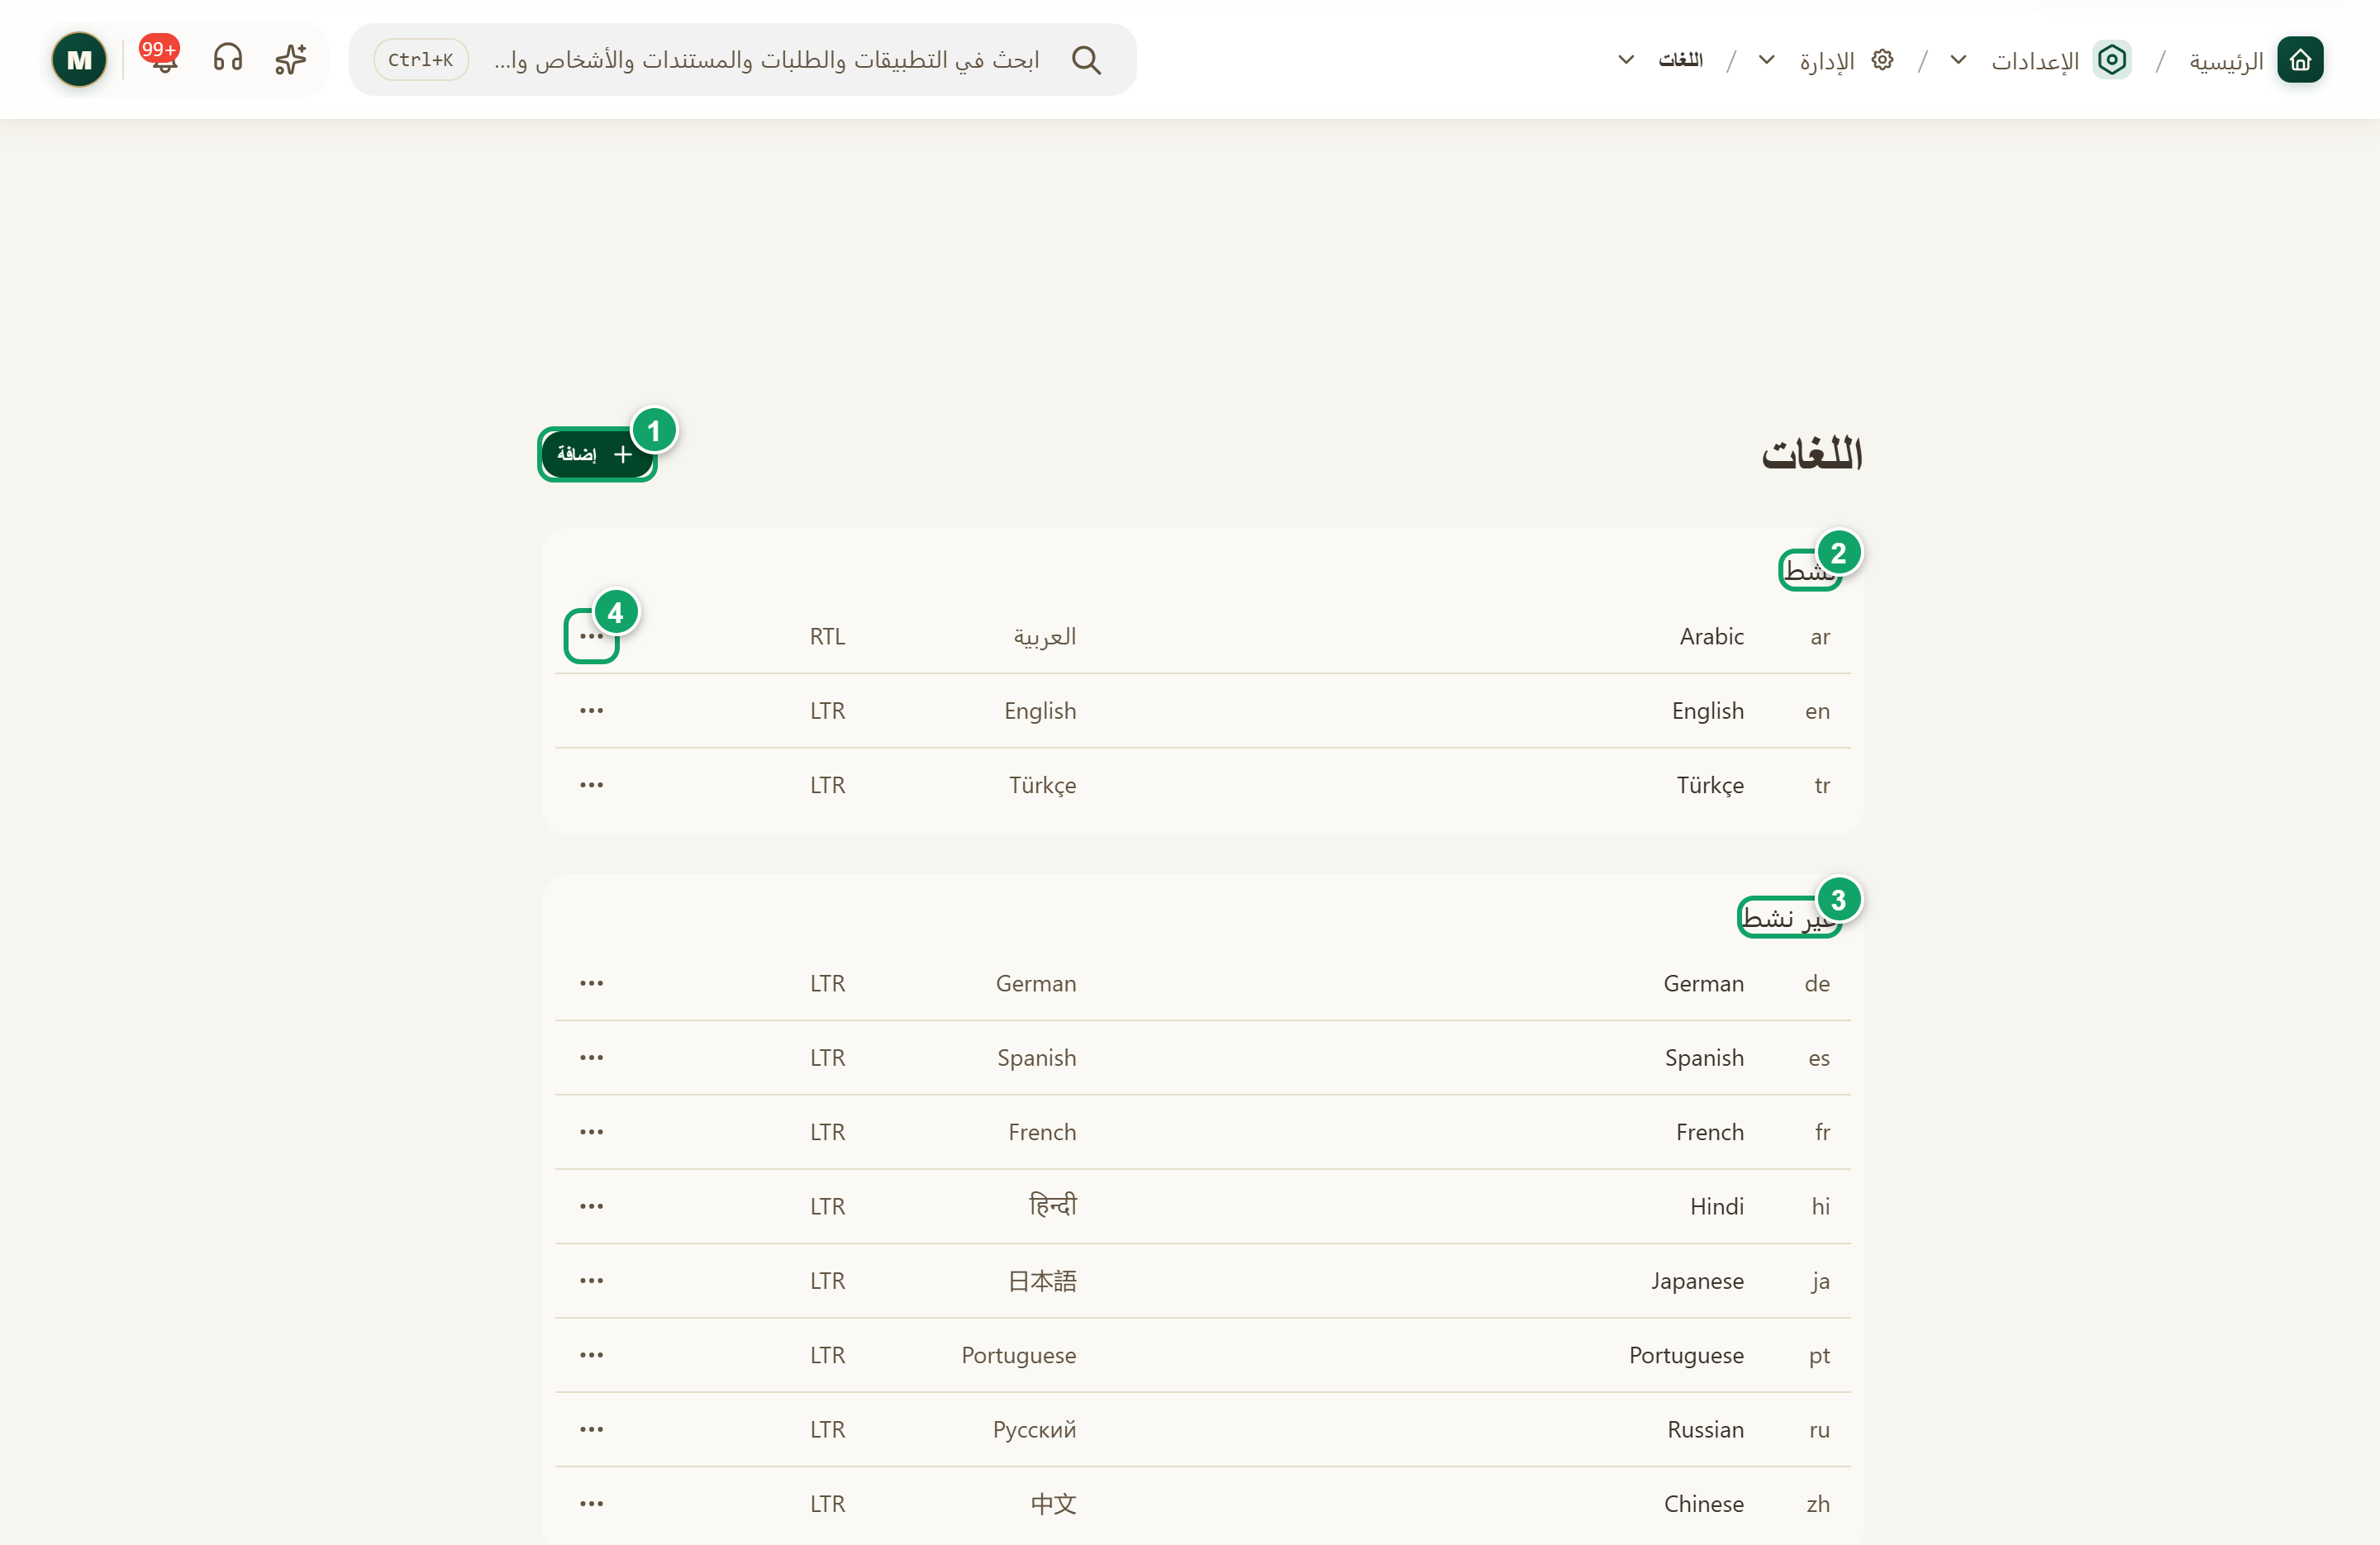
\includegraphics[width=0.95\linewidth,height=0.72\textheight,keepaspectratio]{figures/screens/ch08-languages-ar.png}
\caption{اللغات النشطة وغير النشطة}
\label{fig:settings-languages-screen}
\shotnote{تعرض الصفحة لغات المؤسسة في قائمتين بحسب الحالة، ويبين كل صف رمز اللغة واسمها واسمها المحلي واتجاه كتابتها. والنقل بين القائمتين أسلم من الحذف؛ فهو لا يزيل تعريف اللغة. ① «إضافة». ② «نشط»: اللغات التي تظهر في الحقول متعددة اللغات. ③ «غير نشط»: لغات معرّفة لا تُعرض للكتابة. ④ زر النقاط الثلاث: يفتح «تعديل» و«حذف».}
\end{figure}

\begin{figure}[H]
\centering
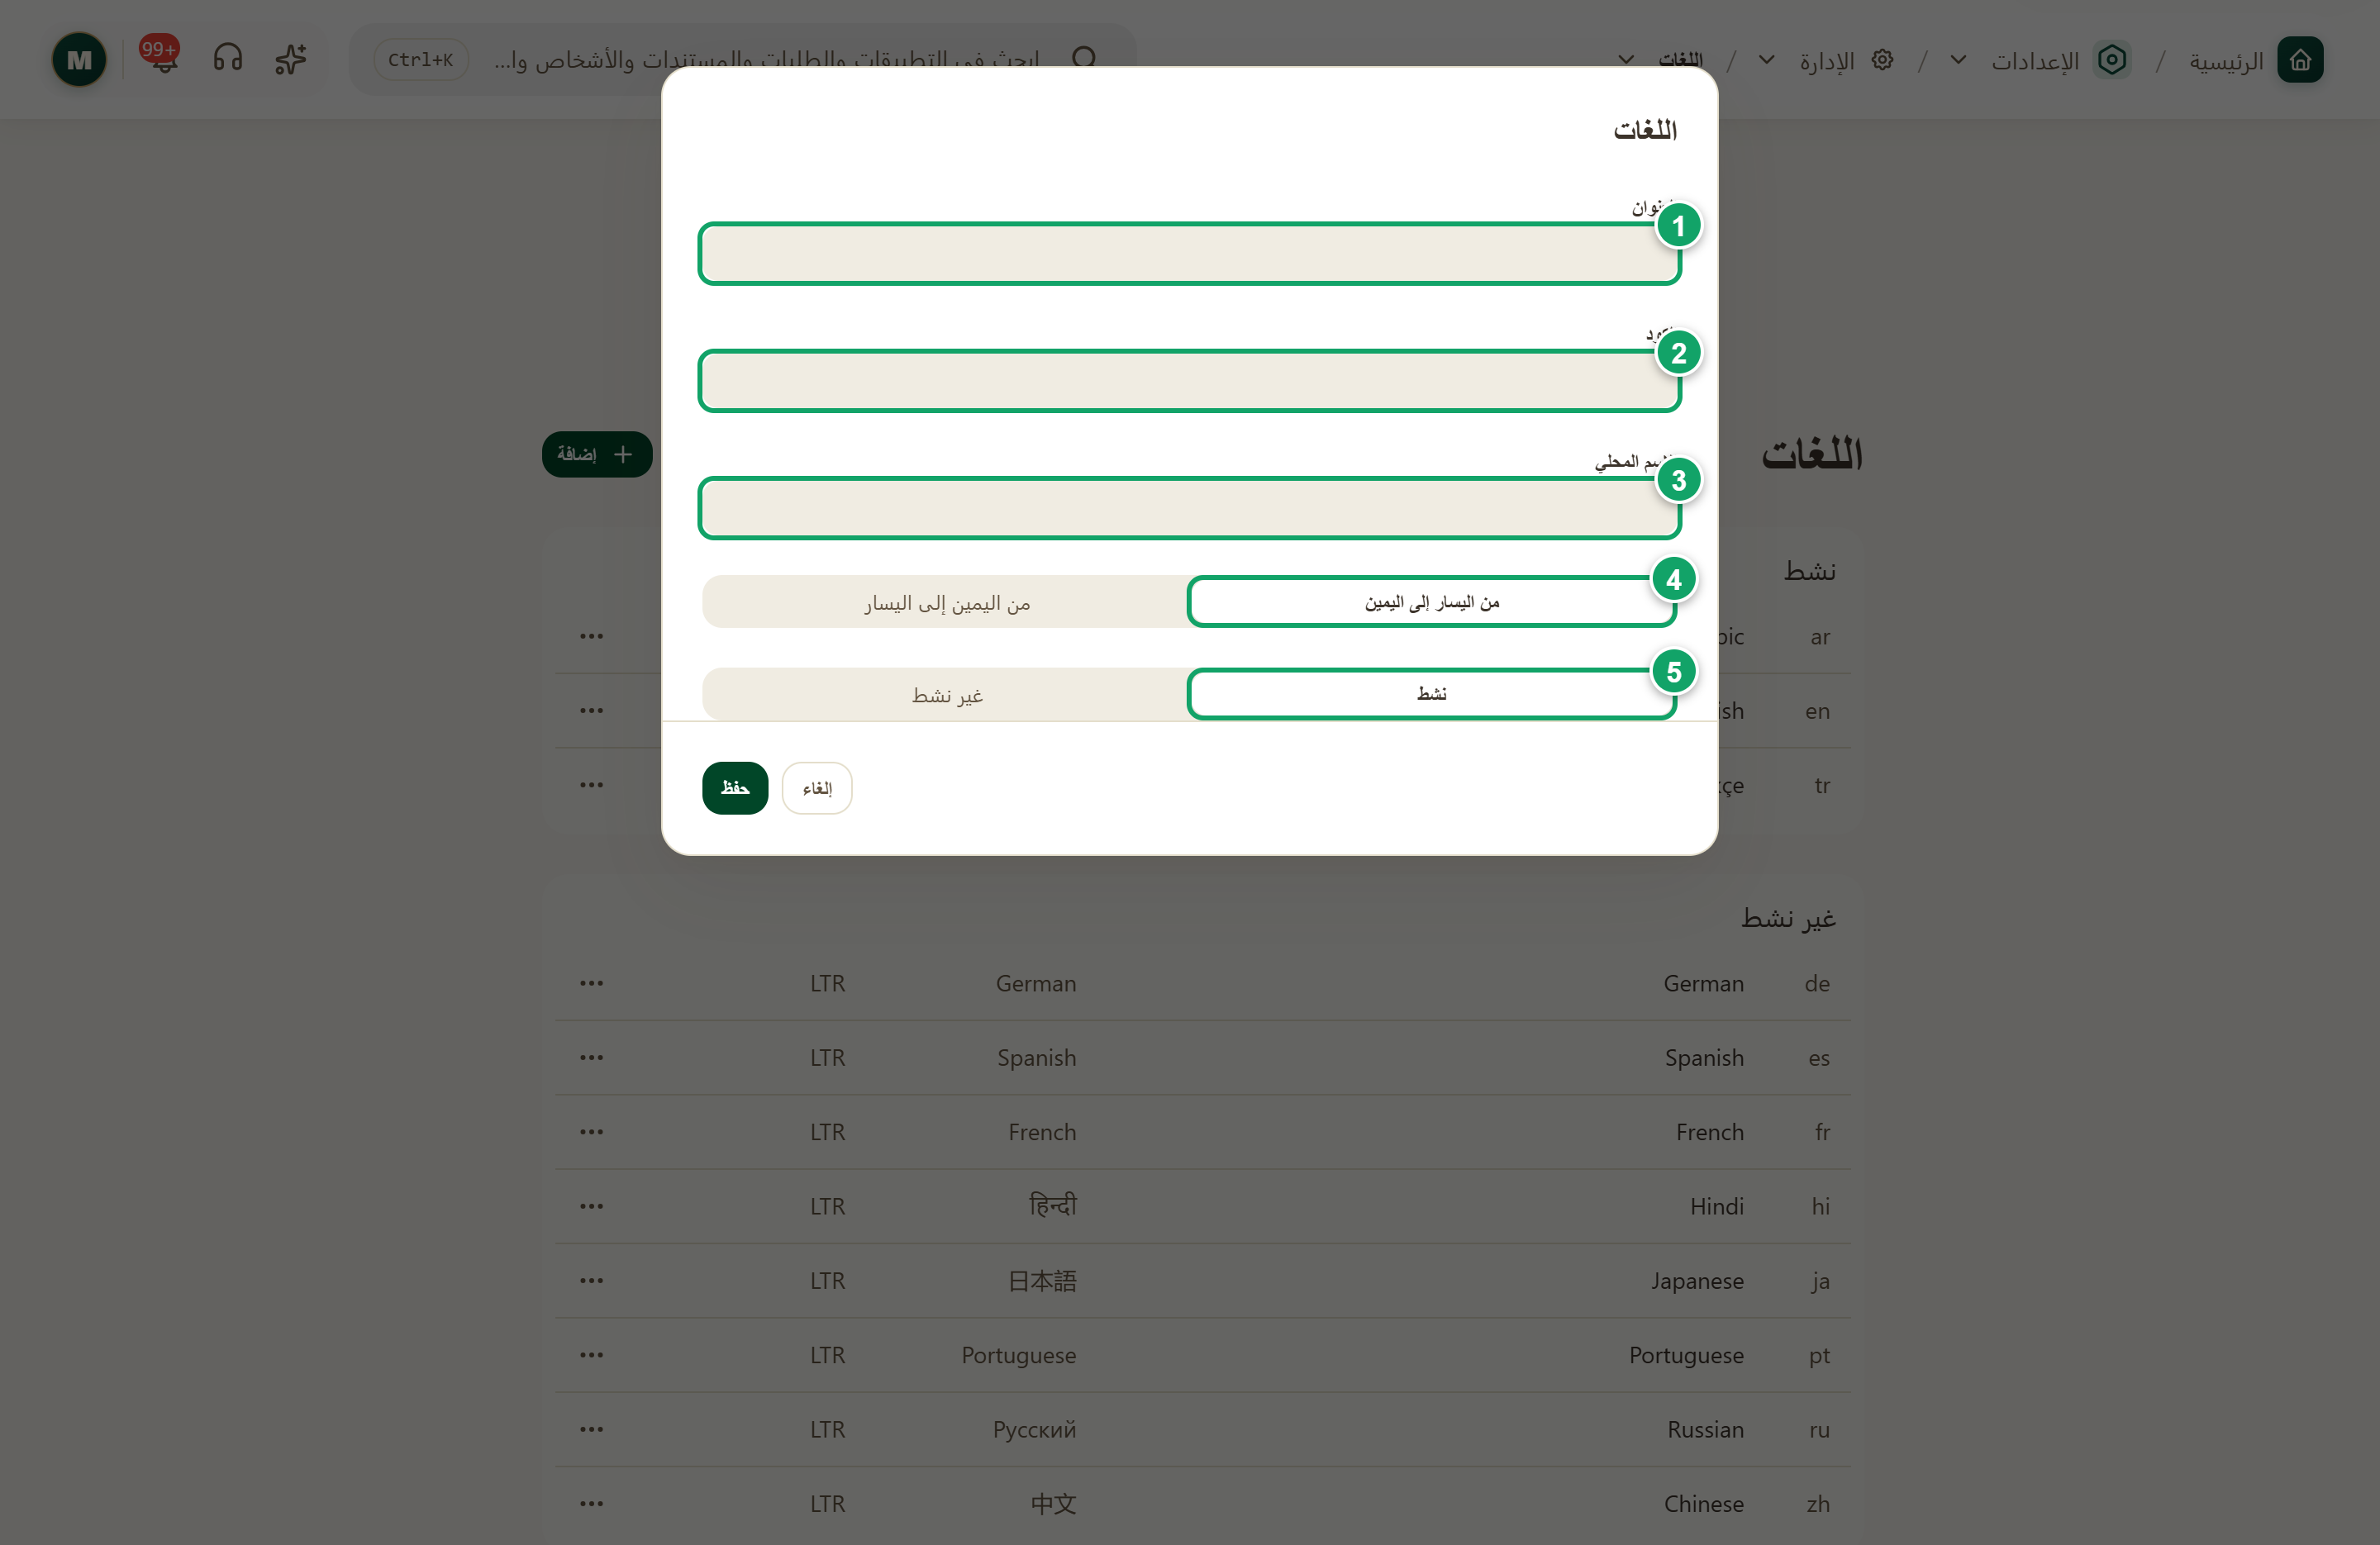
\includegraphics[width=0.95\linewidth,height=0.72\textheight,keepaspectratio]{figures/screens/ch08-languages-form-ar.png}
\caption{نموذج إضافة لغة}
\label{fig:settings-languages-form-screen}
\shotnote{تعرض النافذة الحقول الخمسة التي تعرّف اللغة، وهي فارغة لأنها فُتحت للعرض ولم تُحفظ. يكفي «العنوان» و«الكود» لحفظ اللغة، أما بقية القيم فلها اختيار افتراضي. ① «العنوان». ② «الكود»: رمز قصير مثل \en{ku}، ولا يُقبل رمز مستخدم للغة أخرى. ③ «الاسم المحلي»: اسم اللغة بحروفها. ④ اتجاه الكتابة. ⑤ الحالة.}
\end{figure}

\begin{table}[H]
\centering
\caption{ماذا تسجل في اللغة؟}
\label{tab:settings-languages-fields}
\begin{tabularx}{\linewidth}{R{4.2cm} Y}
\rcHeaderRow
\thh{الحقل} & \thh{ماذا تكتب؟}\\
«العنوان» & اسم اللغة كما تريد ظهوره، وهو مطلوب.\\
«الكود» & رمز اللغة، وهو مطلوب. تُعد الرموز التي لا تختلف إلا في الأحرف الكبيرة والصغيرة أو المسافات لغة واحدة.\\
«الاسم المحلي» & الاسم بلغته الأصلية، مثل «العربية». وهو اختياري.\\
الاتجاه & «من اليسار إلى اليمين» أو «من اليمين إلى اليسار».\\
الحالة & «نشط» لعرض اللغة، و«غير نشط» لإبقائها معرّفة دون عرض.\\
\end{tabularx}
\end{table}

\begin{enumerate}
\item افتح «الإعدادات» ثم «اللغات».
\item اضغط «إضافة»، أو افتح قائمة لغة موجودة واضغط «تعديل».
\item اكتب «العنوان» و«الكود» و«الاسم المحلي»، ثم اختر الاتجاه والحالة.
\item اضغط «حفظ». وإذا أردت إيقاف لغة فاجعلها «غير نشط» بدلاً من حذفها.
\end{enumerate}

\textbf{تحقق:} تظهر اللغة في القائمة المطابقة لحالتها. افتح بعد ذلك حقلاً متعدد اللغات، ثم تأكد من ظهور اللغة النشطة فيه. وإذا رُفض الرمز، فستذكر الرسالة اللغة التي تستخدمه.

\section{العملات}
\label{sec:settings-feature-currencies}

تجمع هذه الصفحة ما يحتاج إليه النظام ليتعامل مع المبالغ بأكثر من عملة: قائمة العملات، وأسعار الصرف، ونشرات الأسعار، وأنواع الأسعار، وقواعد التقريب والعرض. وأهم مفهوم فيها «العملة الأساسية»، وهي العملة التي يُحفظ بها مكافئ كل مبلغ لتُجمع المبالغ المختلفة في القوائم والتقارير. يفتح الصفحة من يملك صلاحية العملات، أما تغيير «إعدادات المبالغ» وأنواع الأسعار فمقصور على مالك المؤسسة وحاملي دور المسؤول.

\begin{rcnote}[مثال: شركة الأفق]
تحاسب شركة الأفق بالليرة السورية وتستلم بعض الدفعات بالدولار. فيجعل مسؤول النظام الليرة عملة أساسية، ويفعّل الدولار، ثم يضغط «إضافة سعر» كل صباح لتسجيل سعر السوق.
\end{rcnote}

\begin{figure}[H]
\centering
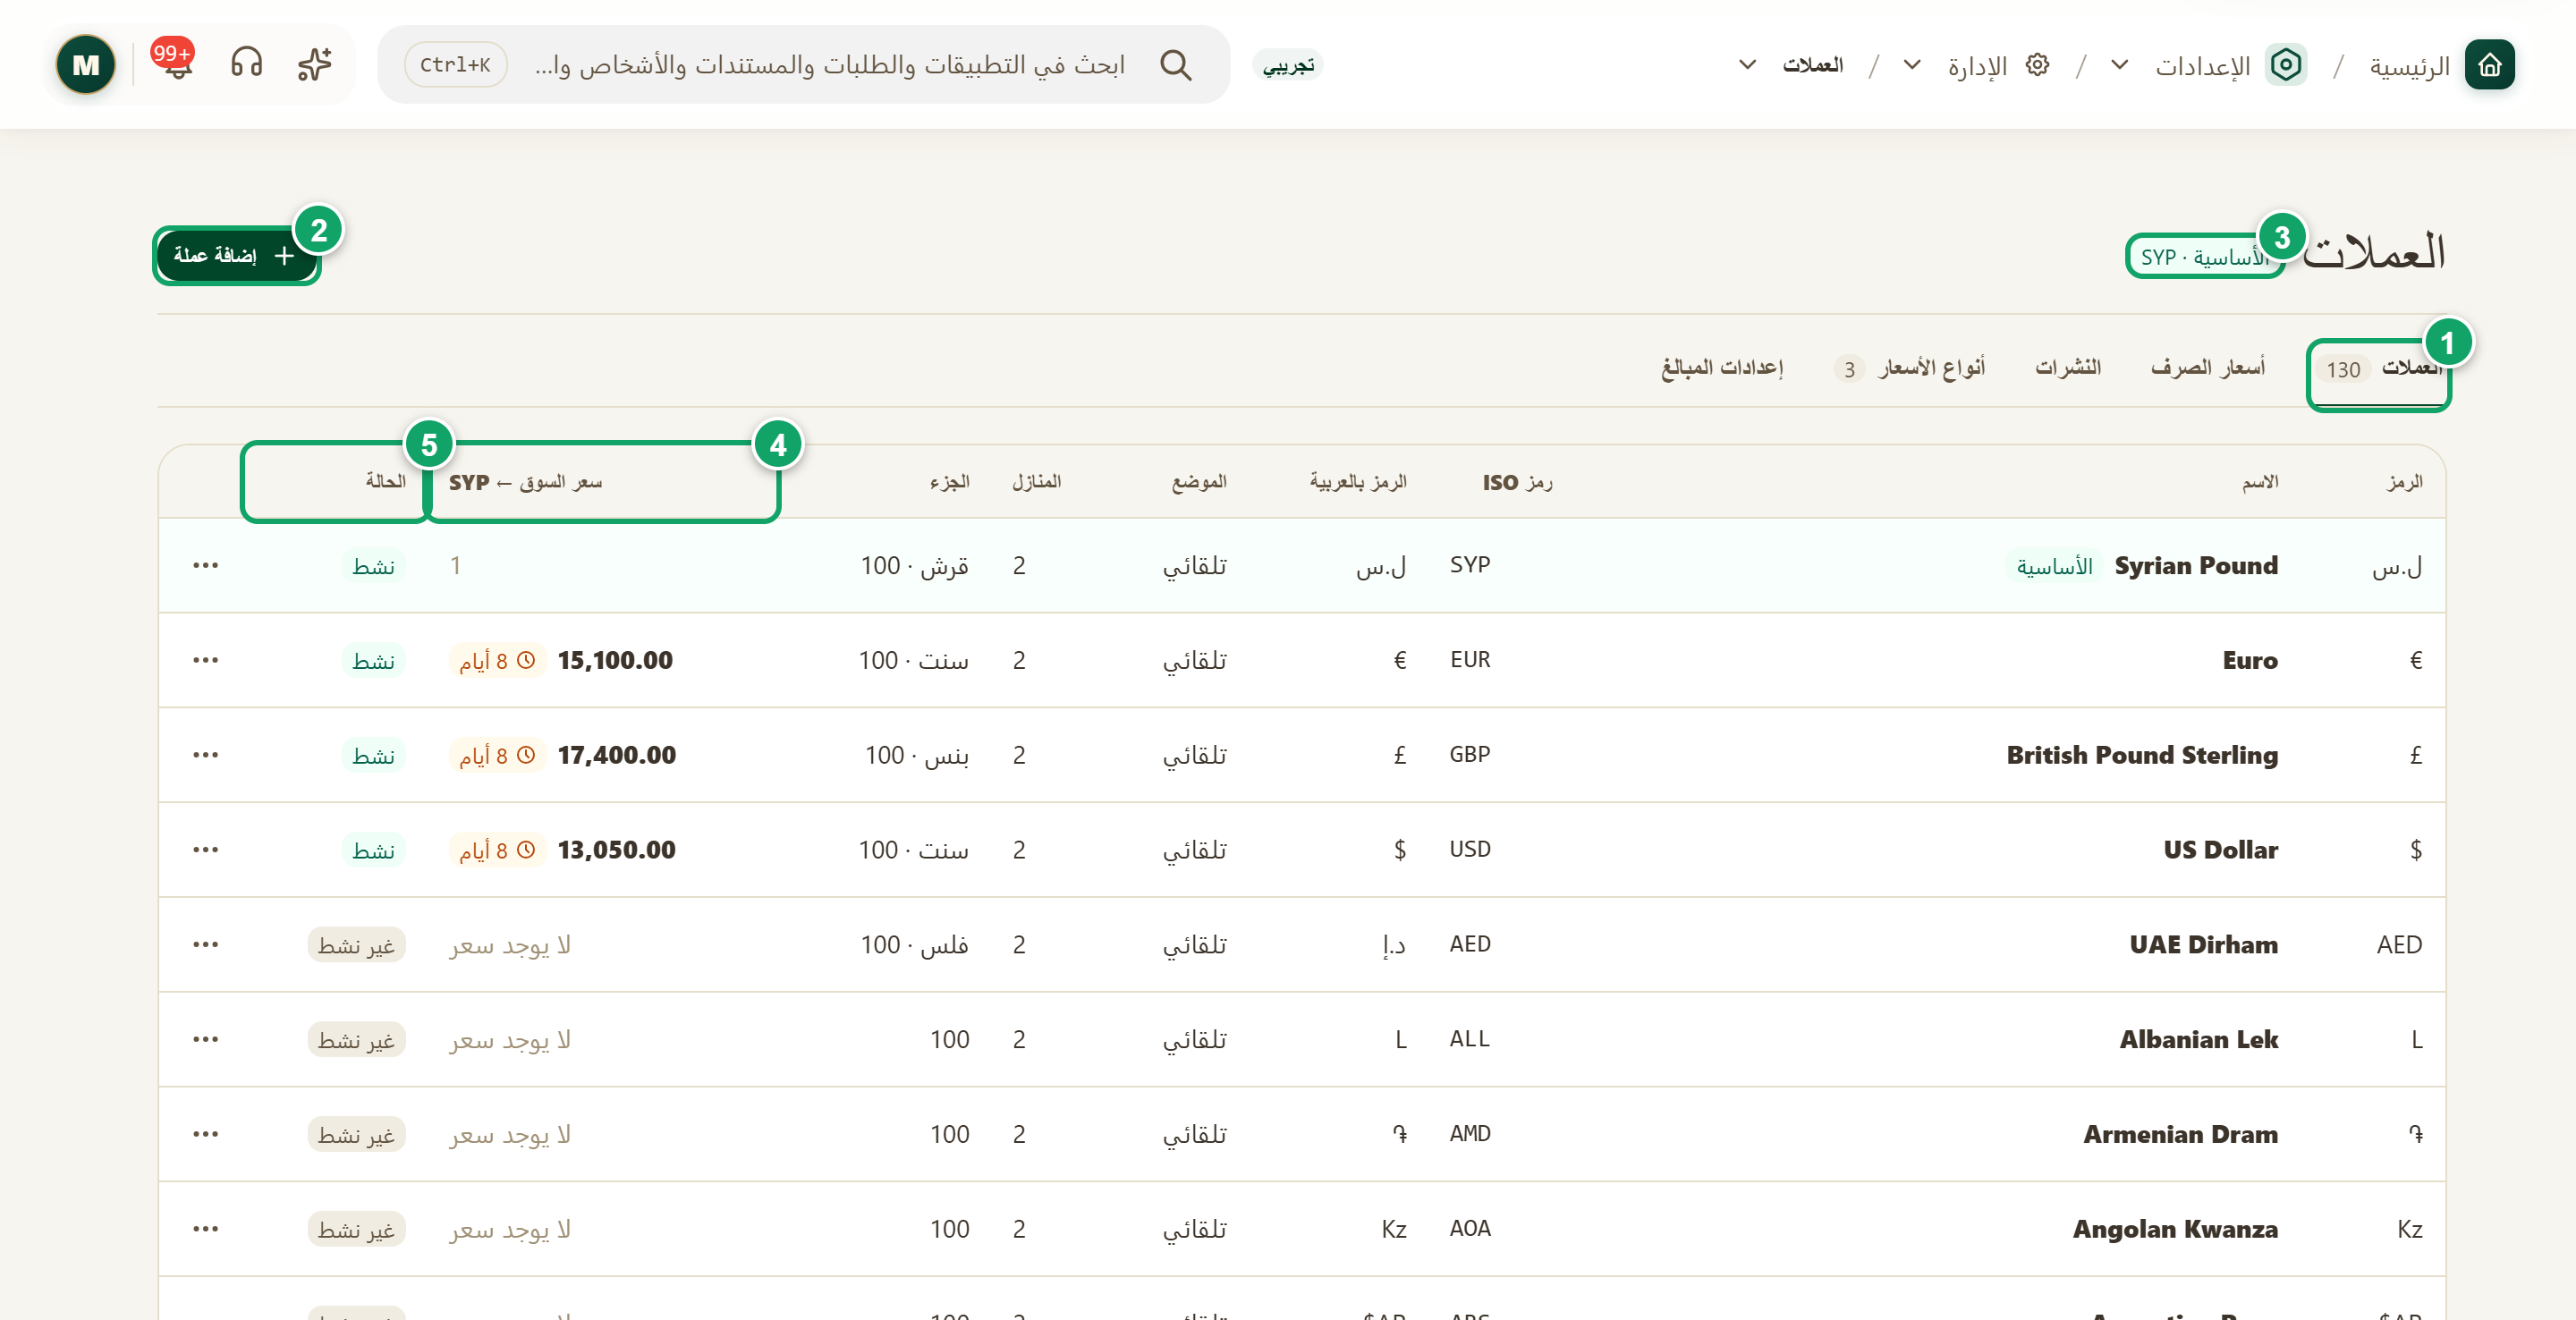
\includegraphics[width=0.95\linewidth,height=0.72\textheight,keepaspectratio]{figures/screens/ch08-currencies-ar.png}
\caption{قائمة العملات}
\label{fig:settings-currencies-screen}
\shotnote{تعرض القائمة كل عملة ورموزها ومنازلها العشرية وآخر سعر لها مقابل العملة الأساسية. ولا تُختار في القيم الجديدة إلا العملات النشطة، أما المبالغ المحفوظة بعملة أوقفتها فتبقى ظاهرة. ① «العملات». ② «إضافة عملة». ③ شارة «الأساسية»: تعرض رمز العملة الأساسية للمؤسسة. ④ عمود السعر: آخر سعر من نوع السعر الافتراضي، وبجانبه عدد أيامه إذا أصبح قديماً. ⑤ «الحالة».}
\end{figure}

\begin{table}[H]
\centering
\caption{ماذا تسجل في العملة؟}
\label{tab:settings-currencies-fields}
\begin{tabularx}{\linewidth}{R{4.2cm} Y}
\rcHeaderRow
\thh{تبويب النافذة} & \thh{ماذا تسجل فيه؟}\\
«عام» & «رمز \en{ISO}» المكوّن من ثلاثة أحرف، و«الرمز»، و«الرمز بالعربية»، و«الاسم»، و«موضع الرمز»، و«المنازل العشرية»، و«الحالة». يثبت رمز \en{ISO} بعد استخدام العملة، ويمكن زيادة المنازل فقط ما دامت هناك مبالغ.\\
«الوحدات والتفقيط» & «نسبة الجزء»، مثل 100 قرش في الليرة، وأسماء الوحدة التي تُستخدم عند كتابة المبلغ بالحروف.\\
«الفئات» & وحدة قديمة للعملة نفسها، مثل حذف الأصفار: 100 قديمة = 1 جديدة. وتُحفظ المبالغ دائماً بالوحدة الحالية.\\
\end{tabularx}
\end{table}

\begin{figure}[H]
\centering
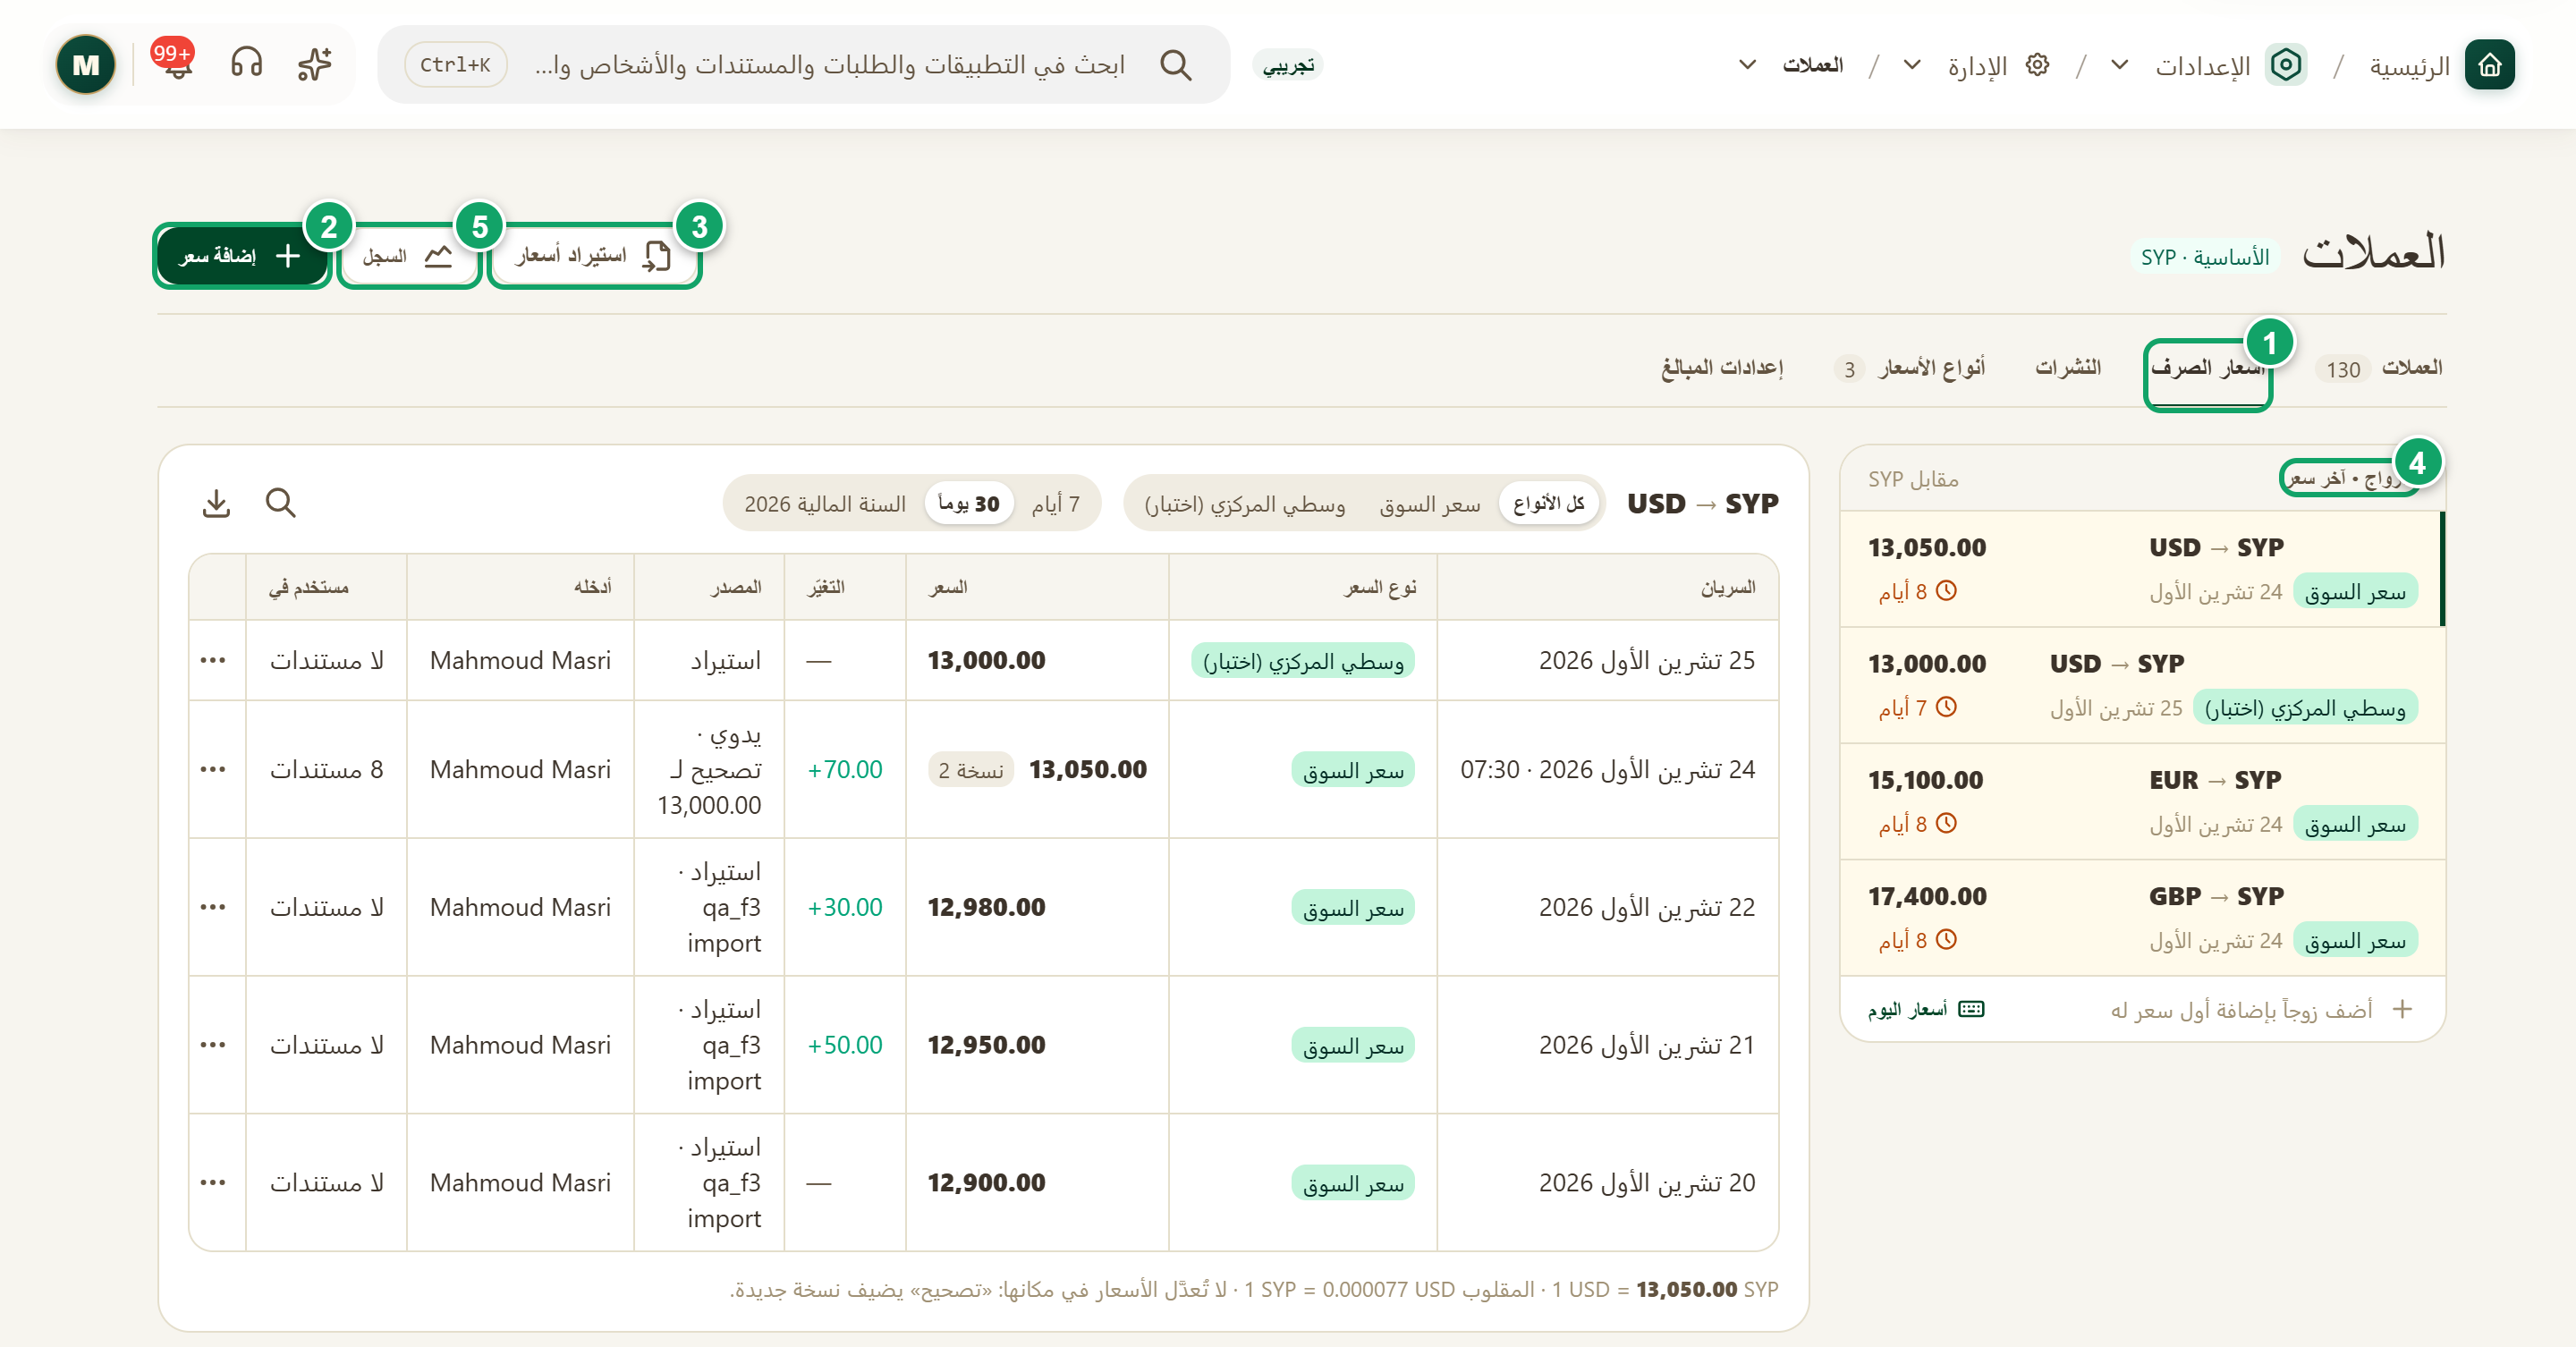
\includegraphics[width=0.95\linewidth,height=0.72\textheight,keepaspectratio]{figures/screens/ch08-currencies-rates-ar.png}
\caption{أسعار الصرف}
\label{fig:settings-currencies-rates-screen}
\shotnote{يعرض التبويب أزواج العملات مع آخر سعر لكل زوج، وسجل الأسعار للزوج المختار. والأسعار لا تُعدَّل في مكانها؛ فأمر «تصحيح…» يضيف نسخة جديدة ويبقي الأصل في السجل، لذلك تعرف دائماً من أدخل السعر ومن أين جاء. ① «أسعار الصرف». ② «إضافة سعر»: تحدد فيه نوع السعر والعملتين والتاريخ والسعر. ③ «استيراد أسعار»: لرفع عدة أسعار من ملف. ④ «الأزواج · آخر سعر»: اختر زوجاً لعرض سجله. ⑤ «السجل»: يعرض تطور السعر في مخطط.}
\end{figure}

\begin{figure}[H]
\centering
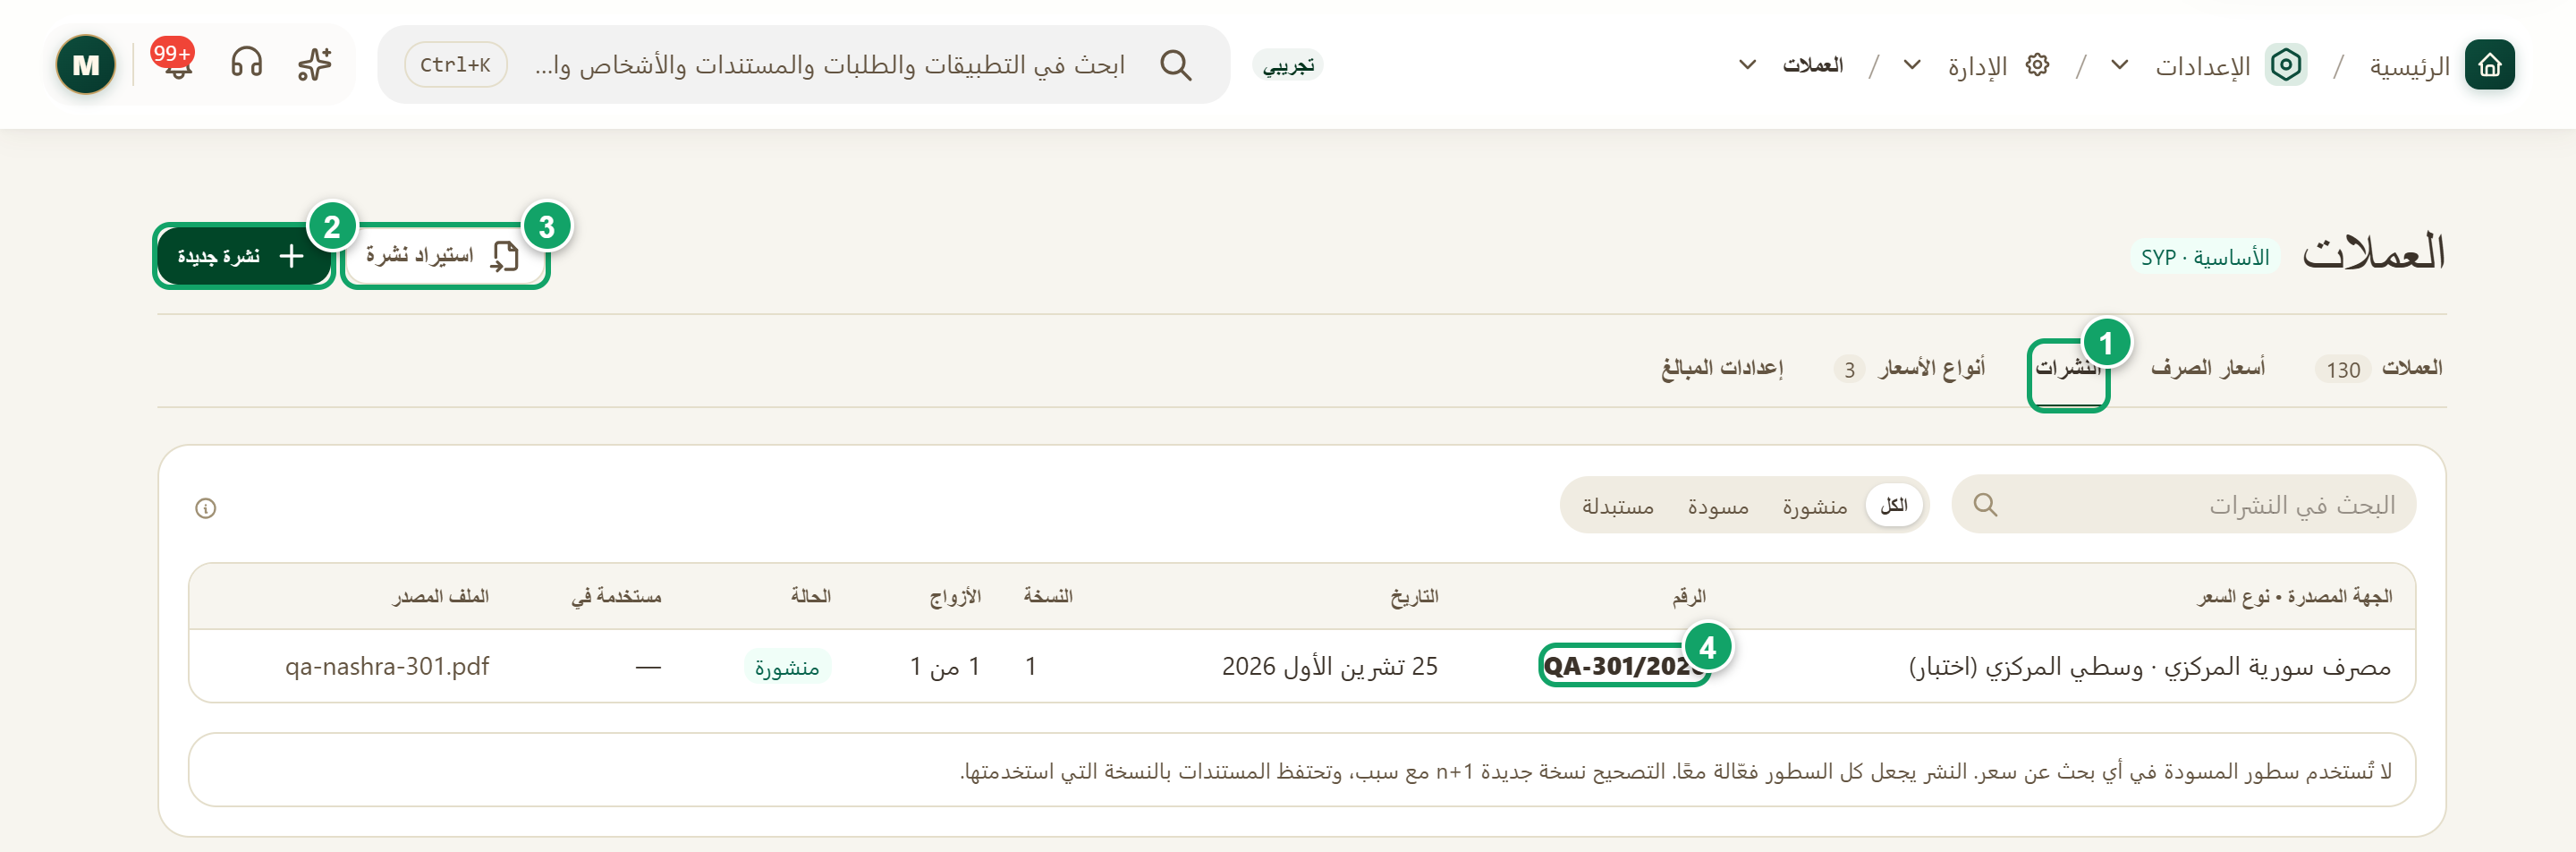
\includegraphics[width=0.95\linewidth,height=0.72\textheight,keepaspectratio]{figures/screens/ch08-currencies-bulletins-ar.png}
\caption{نشرات الأسعار}
\label{fig:settings-currencies-bulletins-screen}
\shotnote{النشرة مجموعة أسعار مؤرخة ومرقمة من جهة واحدة، مثل المصرف المركزي. ولا يقرأ النظام مسودتها، فإذا نُشرت أصبحت كل سطورها فعّالة معاً، ولا تتغير النشرة بعد ذلك إلا بنسخة تصحيح لها سبب. ① «النشرات». ② «نشرة جديدة». ③ «استيراد نشرة». ④ رقم النشرة: افتحه لقراءة سطورها.}
\end{figure}

\begin{figure}[H]
\centering
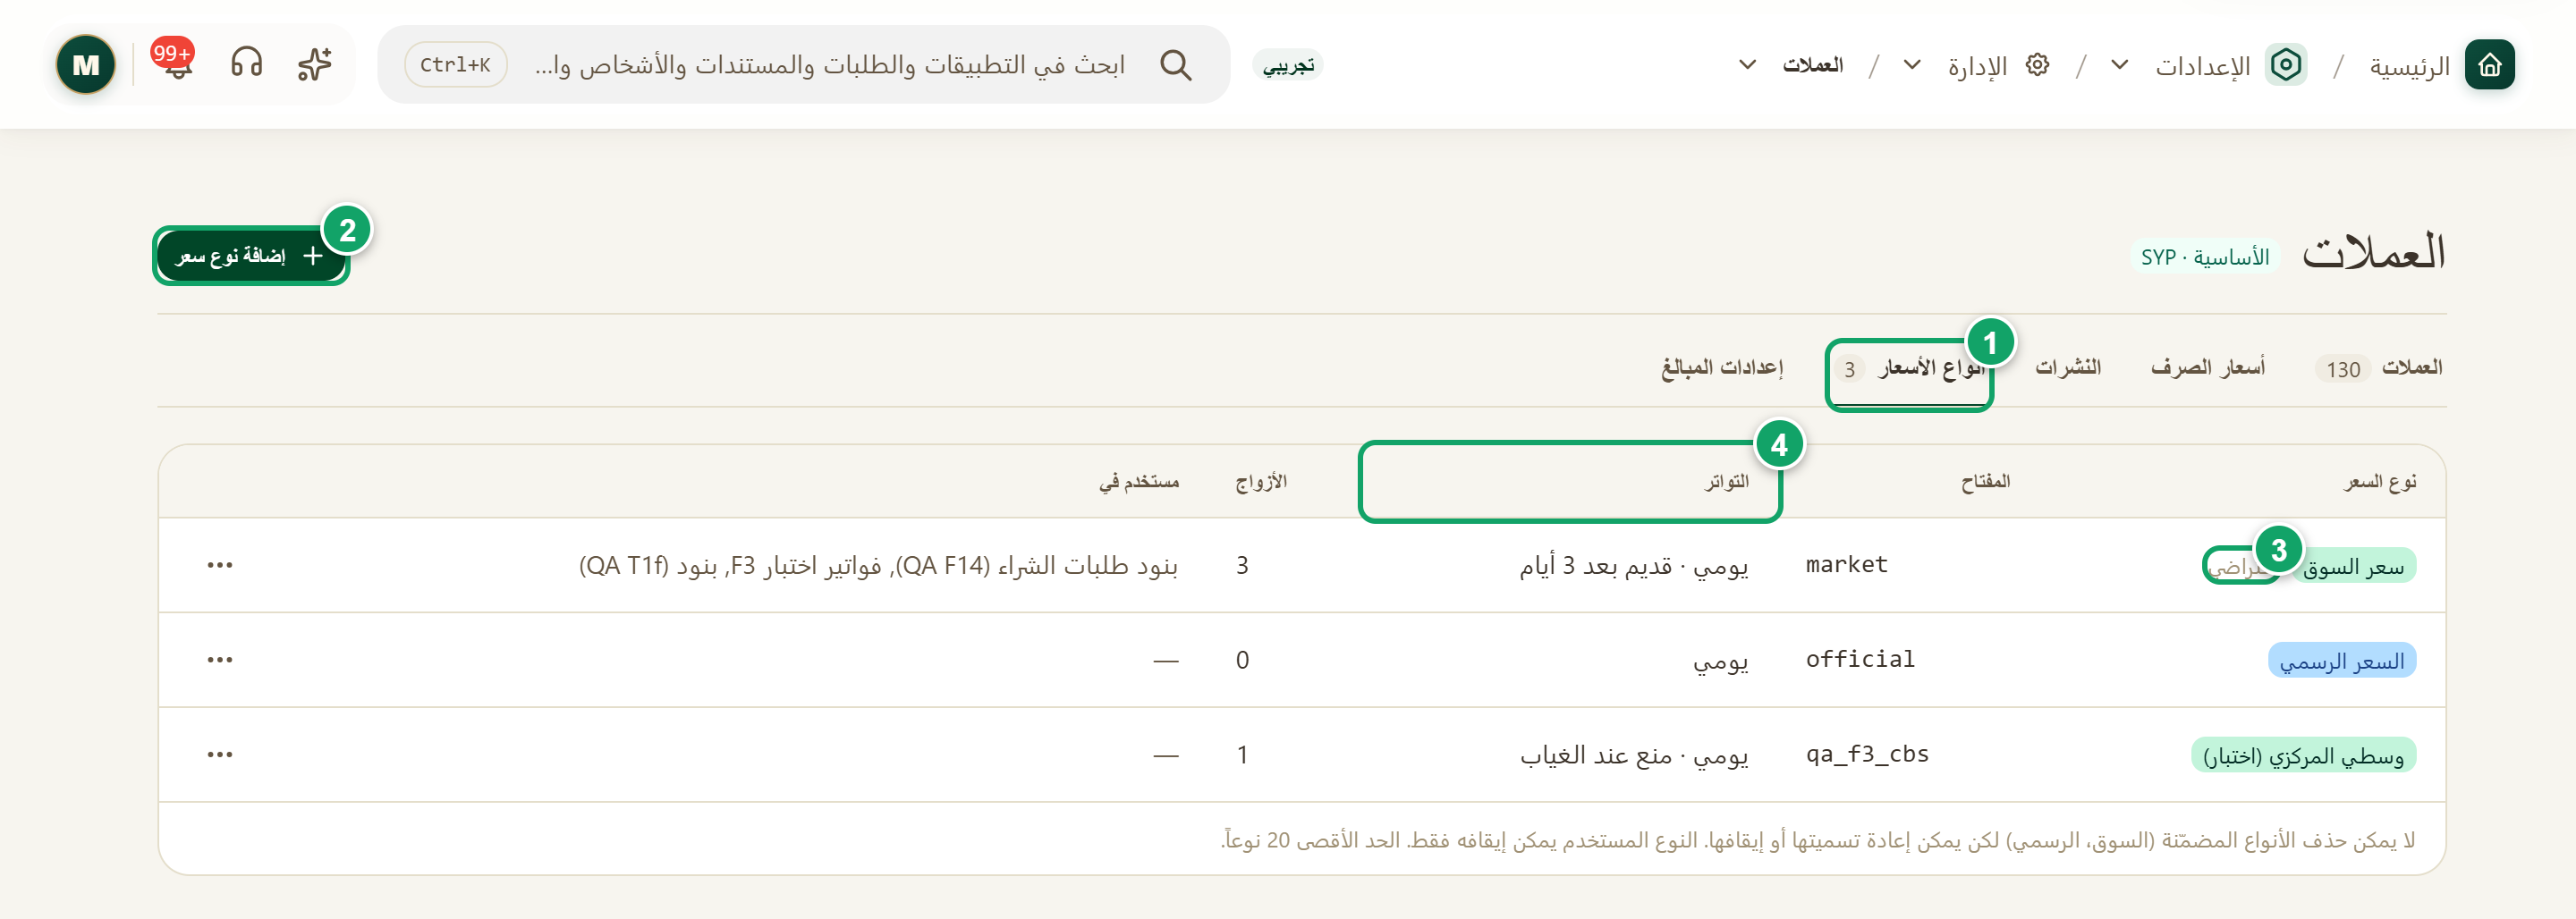
\includegraphics[width=0.95\linewidth,height=0.72\textheight,keepaspectratio]{figures/screens/ch08-currencies-rate-types-ar.png}
\caption{أنواع الأسعار}
\label{fig:settings-currencies-rate-types-screen}
\shotnote{نوع السعر مصدر مسمّى للأسعار، مثل سعر السوق أو تعميم مصرف. وتفيدك الأنواع إذا كان للعملة نفسها أكثر من سعر في اليوم نفسه. ① «أنواع الأسعار». ② «إضافة نوع سعر». ③ «افتراضي»: النوع المستخدم حين لا يختار المستند نوعاً. ④ «التواتر»: كم مرة يُنتظر تحديث السعر، ومتى يُعد قديماً.}
\end{figure}

\begin{figure}[H]
\centering
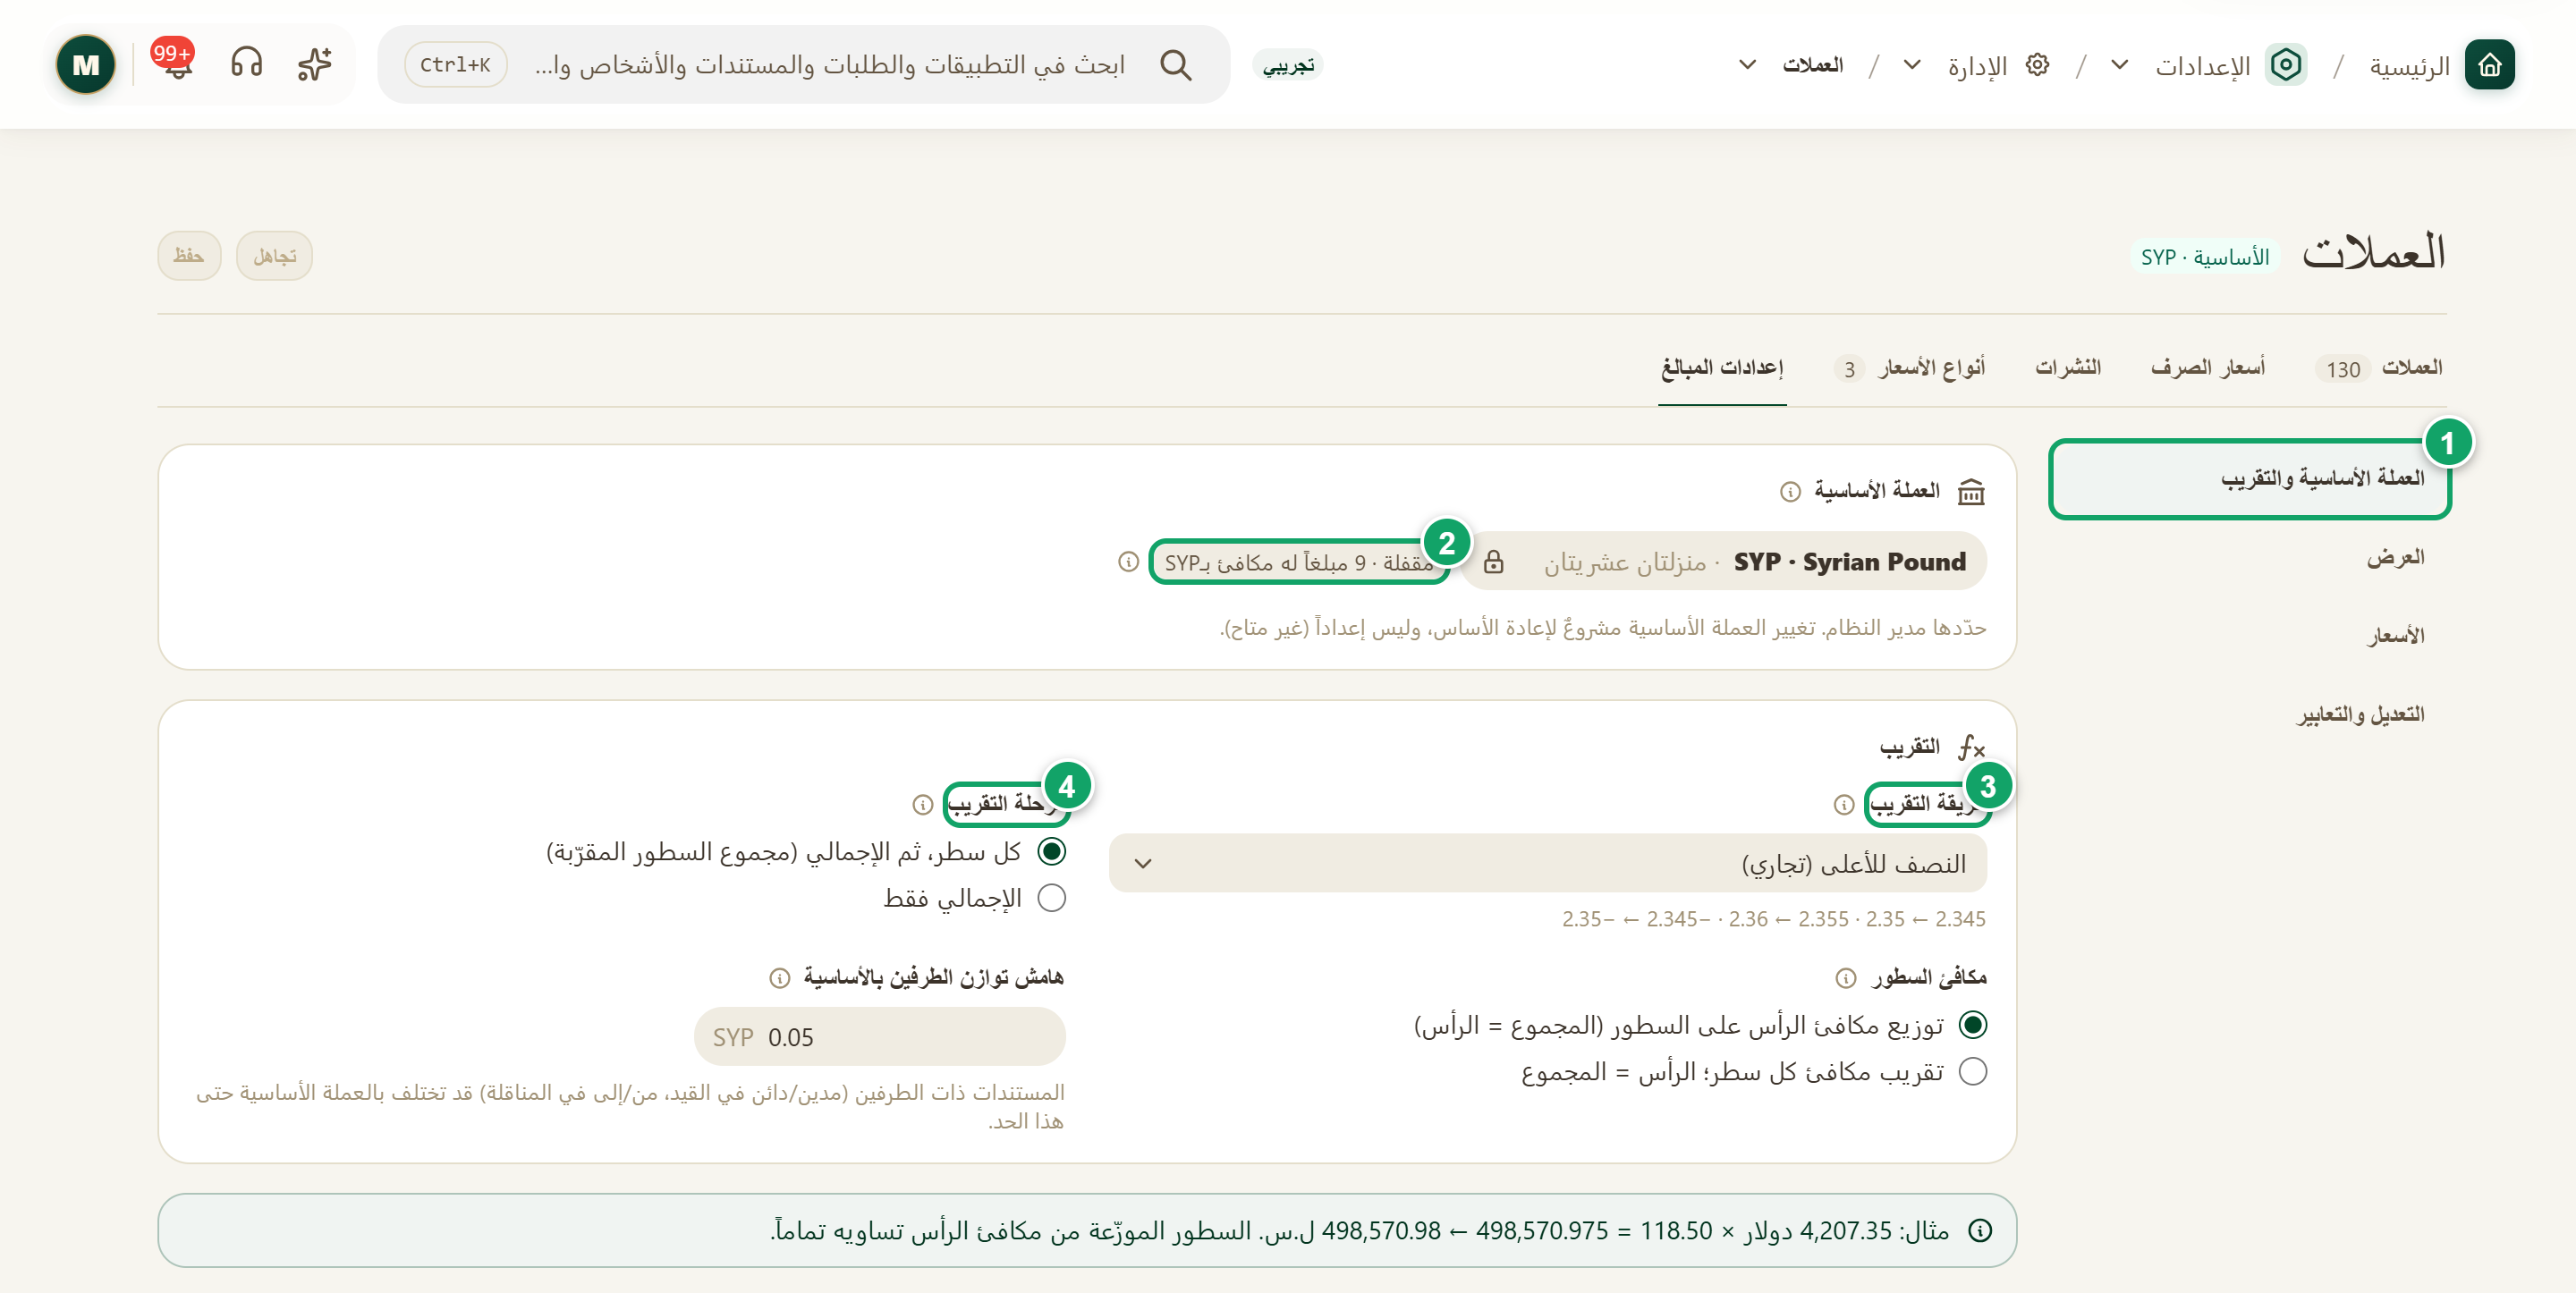
\includegraphics[width=0.95\linewidth,height=0.72\textheight,keepaspectratio]{figures/screens/ch08-currencies-settings-ar.png}
\caption{إعدادات المبالغ: العملة الأساسية والتقريب}
\label{fig:settings-currencies-settings-screen}
\shotnote{يحدد هذا القسم العملة الأساسية وطريقة تقريب المبالغ في كل المستندات. والقفل هنا مقصود؛ فبعد أن يحفظ أول مستند مبلغاً مكافئاً بالعملة الأساسية، لا يعود تغييرها متاحاً. ① «العملة الأساسية والتقريب». ② شارة القفل: تبيّن عدد المبالغ التي تعتمد على العملة الأساسية. ③ «طريقة التقريب». ④ «مرحلة التقريب»: تقريب كل سطر ثم الجمع، أو تقريب الإجمالي فقط.}
\end{figure}

\begin{figure}[H]
\centering
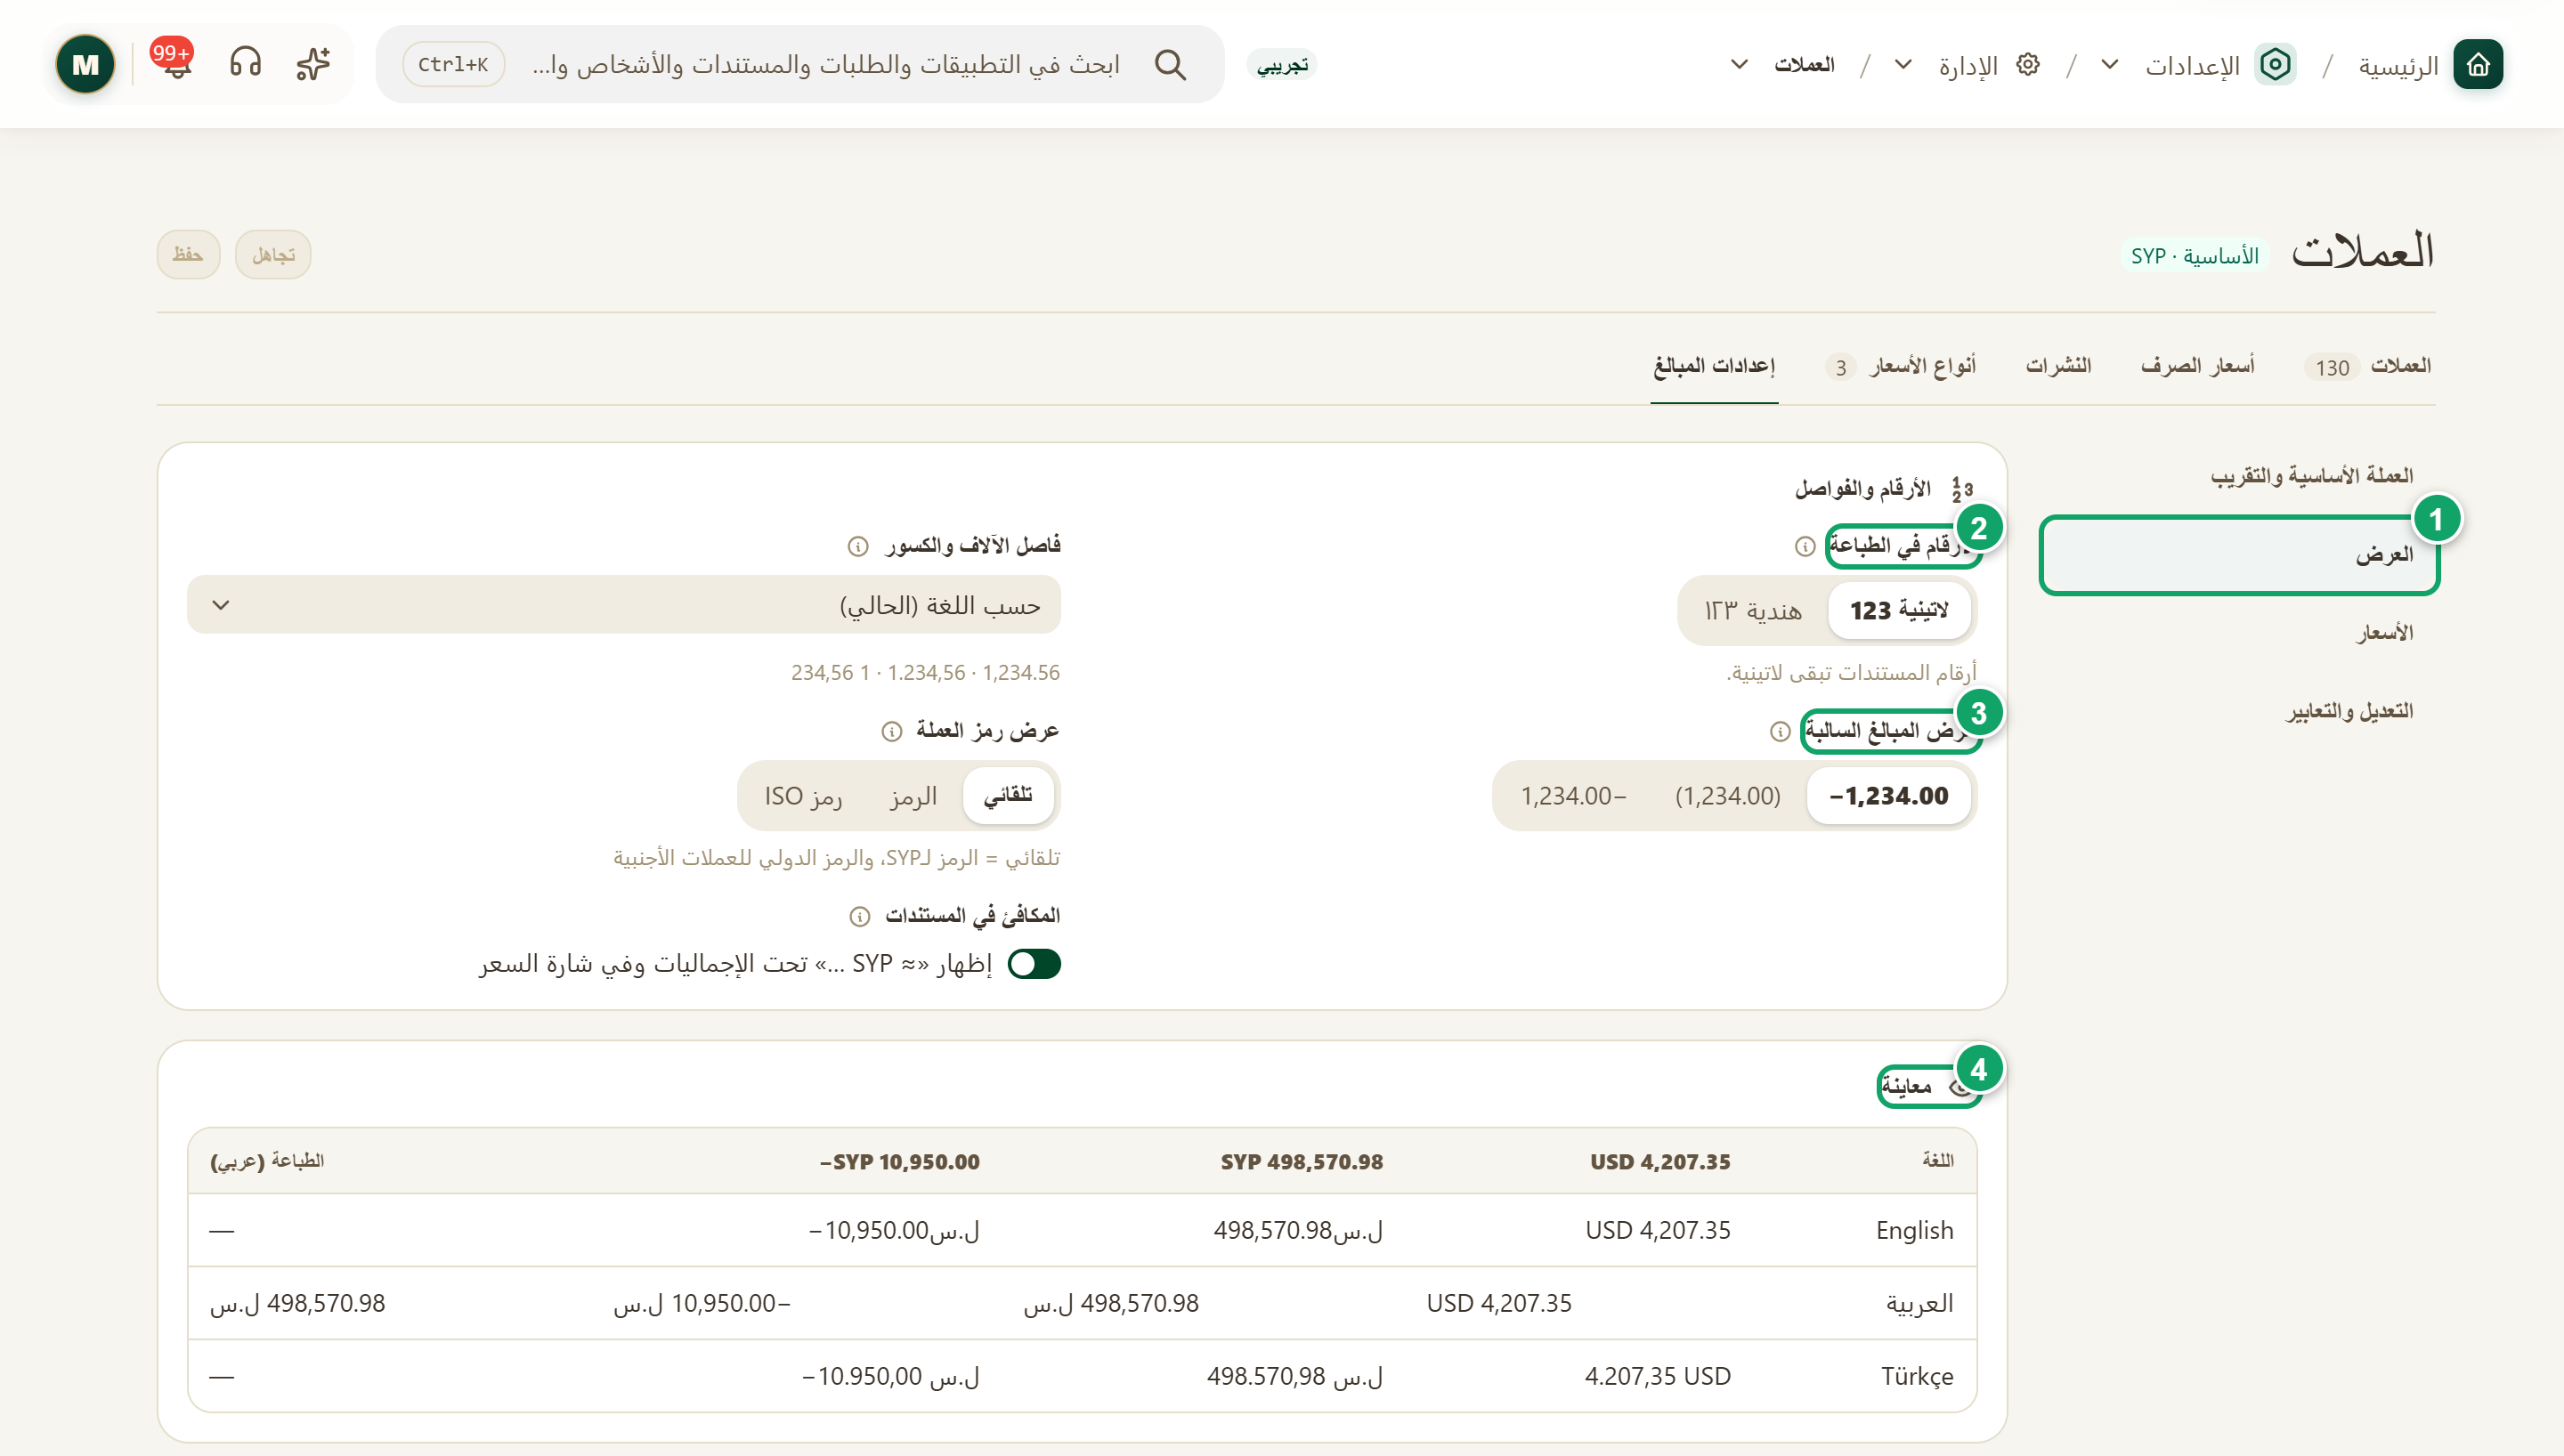
\includegraphics[width=0.95\linewidth,height=0.72\textheight,keepaspectratio]{figures/screens/ch08-currencies-settings-display-ar.png}
\caption{إعدادات المبالغ: العرض}
\label{fig:settings-currencies-settings-display-screen}
\shotnote{يغيّر هذا القسم طريقة قراءة المبالغ فقط، ولا يغيّر قيمها المحفوظة. وتسمح لك المعاينة برؤية الأثر قبل الحفظ بكل لغة نشطة. ① «العرض». ② «الأرقام في الطباعة». ③ «عرض المبالغ السالبة». ④ «معاينة».}
\end{figure}

\begin{figure}[H]
\centering
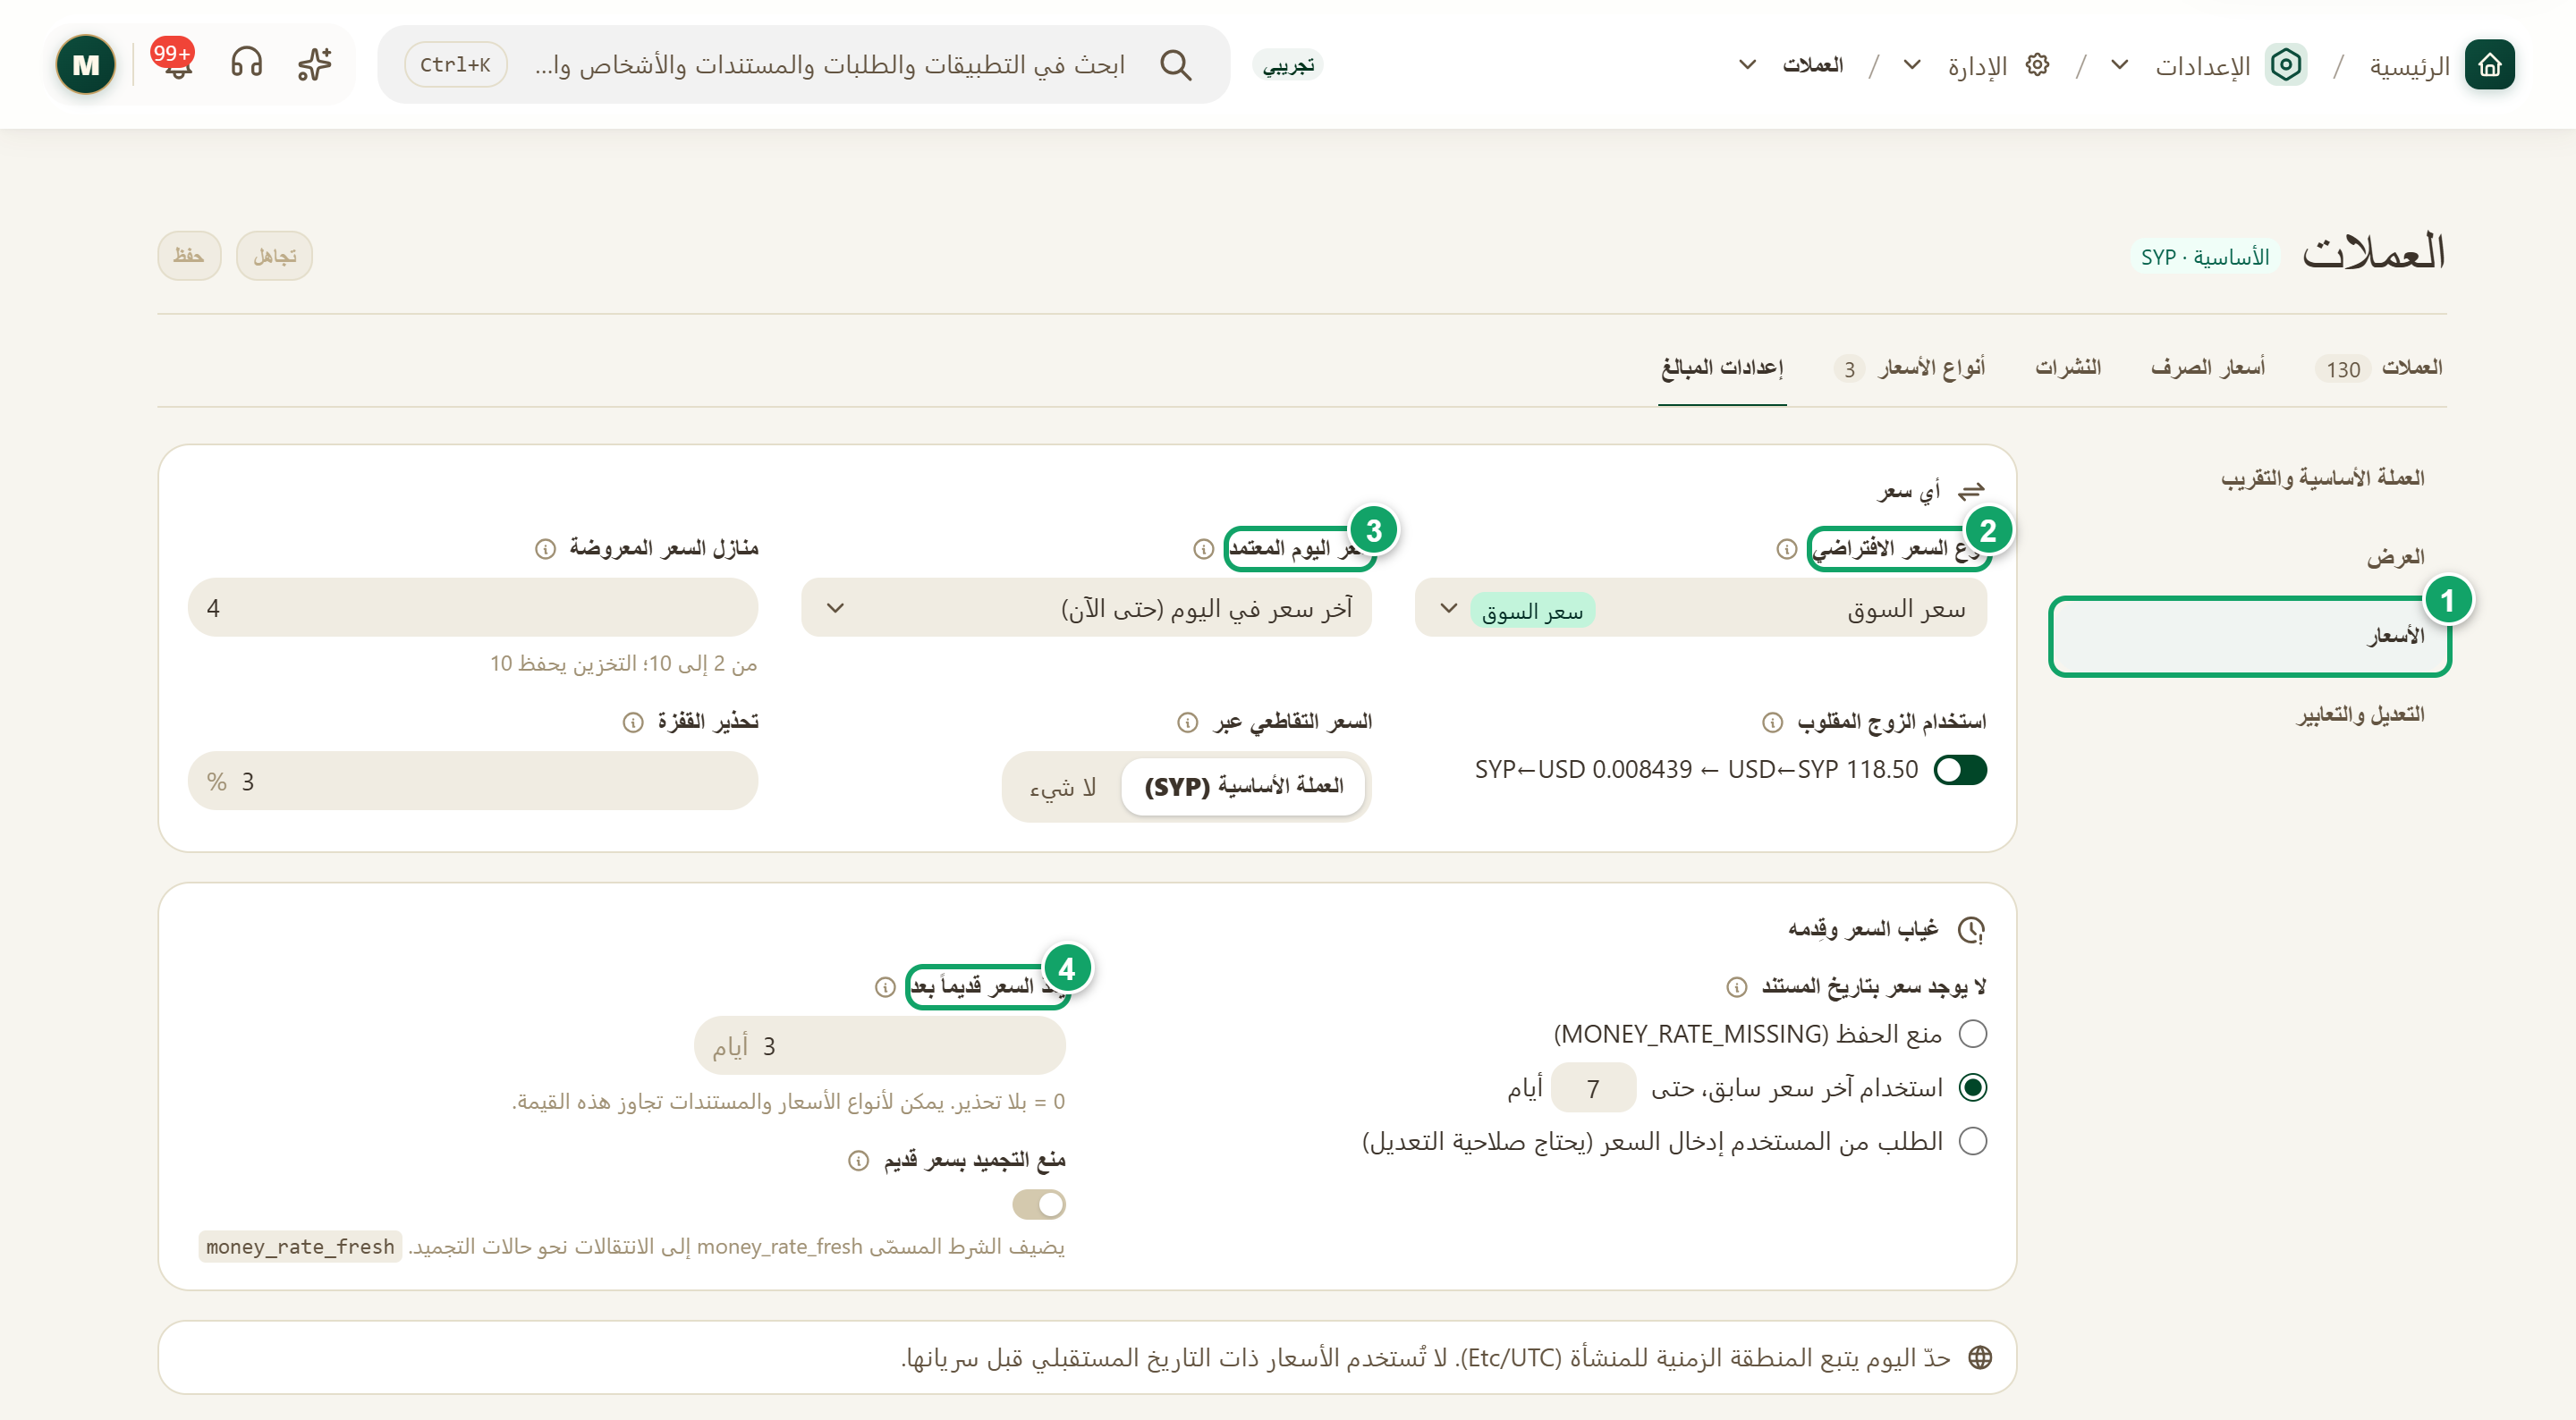
\includegraphics[width=0.95\linewidth,height=0.72\textheight,keepaspectratio]{figures/screens/ch08-currencies-settings-rates-ar.png}
\caption{إعدادات المبالغ: الأسعار}
\label{fig:settings-currencies-settings-rates-screen}
\shotnote{يقرر هذا القسم السعر الذي يختاره النظام للمستند، وما يحدث إذا غاب السعر أو تقادم. وتُحسب بداية اليوم ونهايته بالمنطقة الزمنية للمؤسسة، ولا يُستخدم سعر قبل تاريخ سريانه. ① «الأسعار». ② «نوع السعر الافتراضي». ③ «سعر اليوم المعتمد»: عند وجود أكثر من سعر في اليوم. ④ «يُعدّ السعر قديماً بعد»: الصفر يعني عدم التحذير.}
\end{figure}

\begin{figure}[H]
\centering
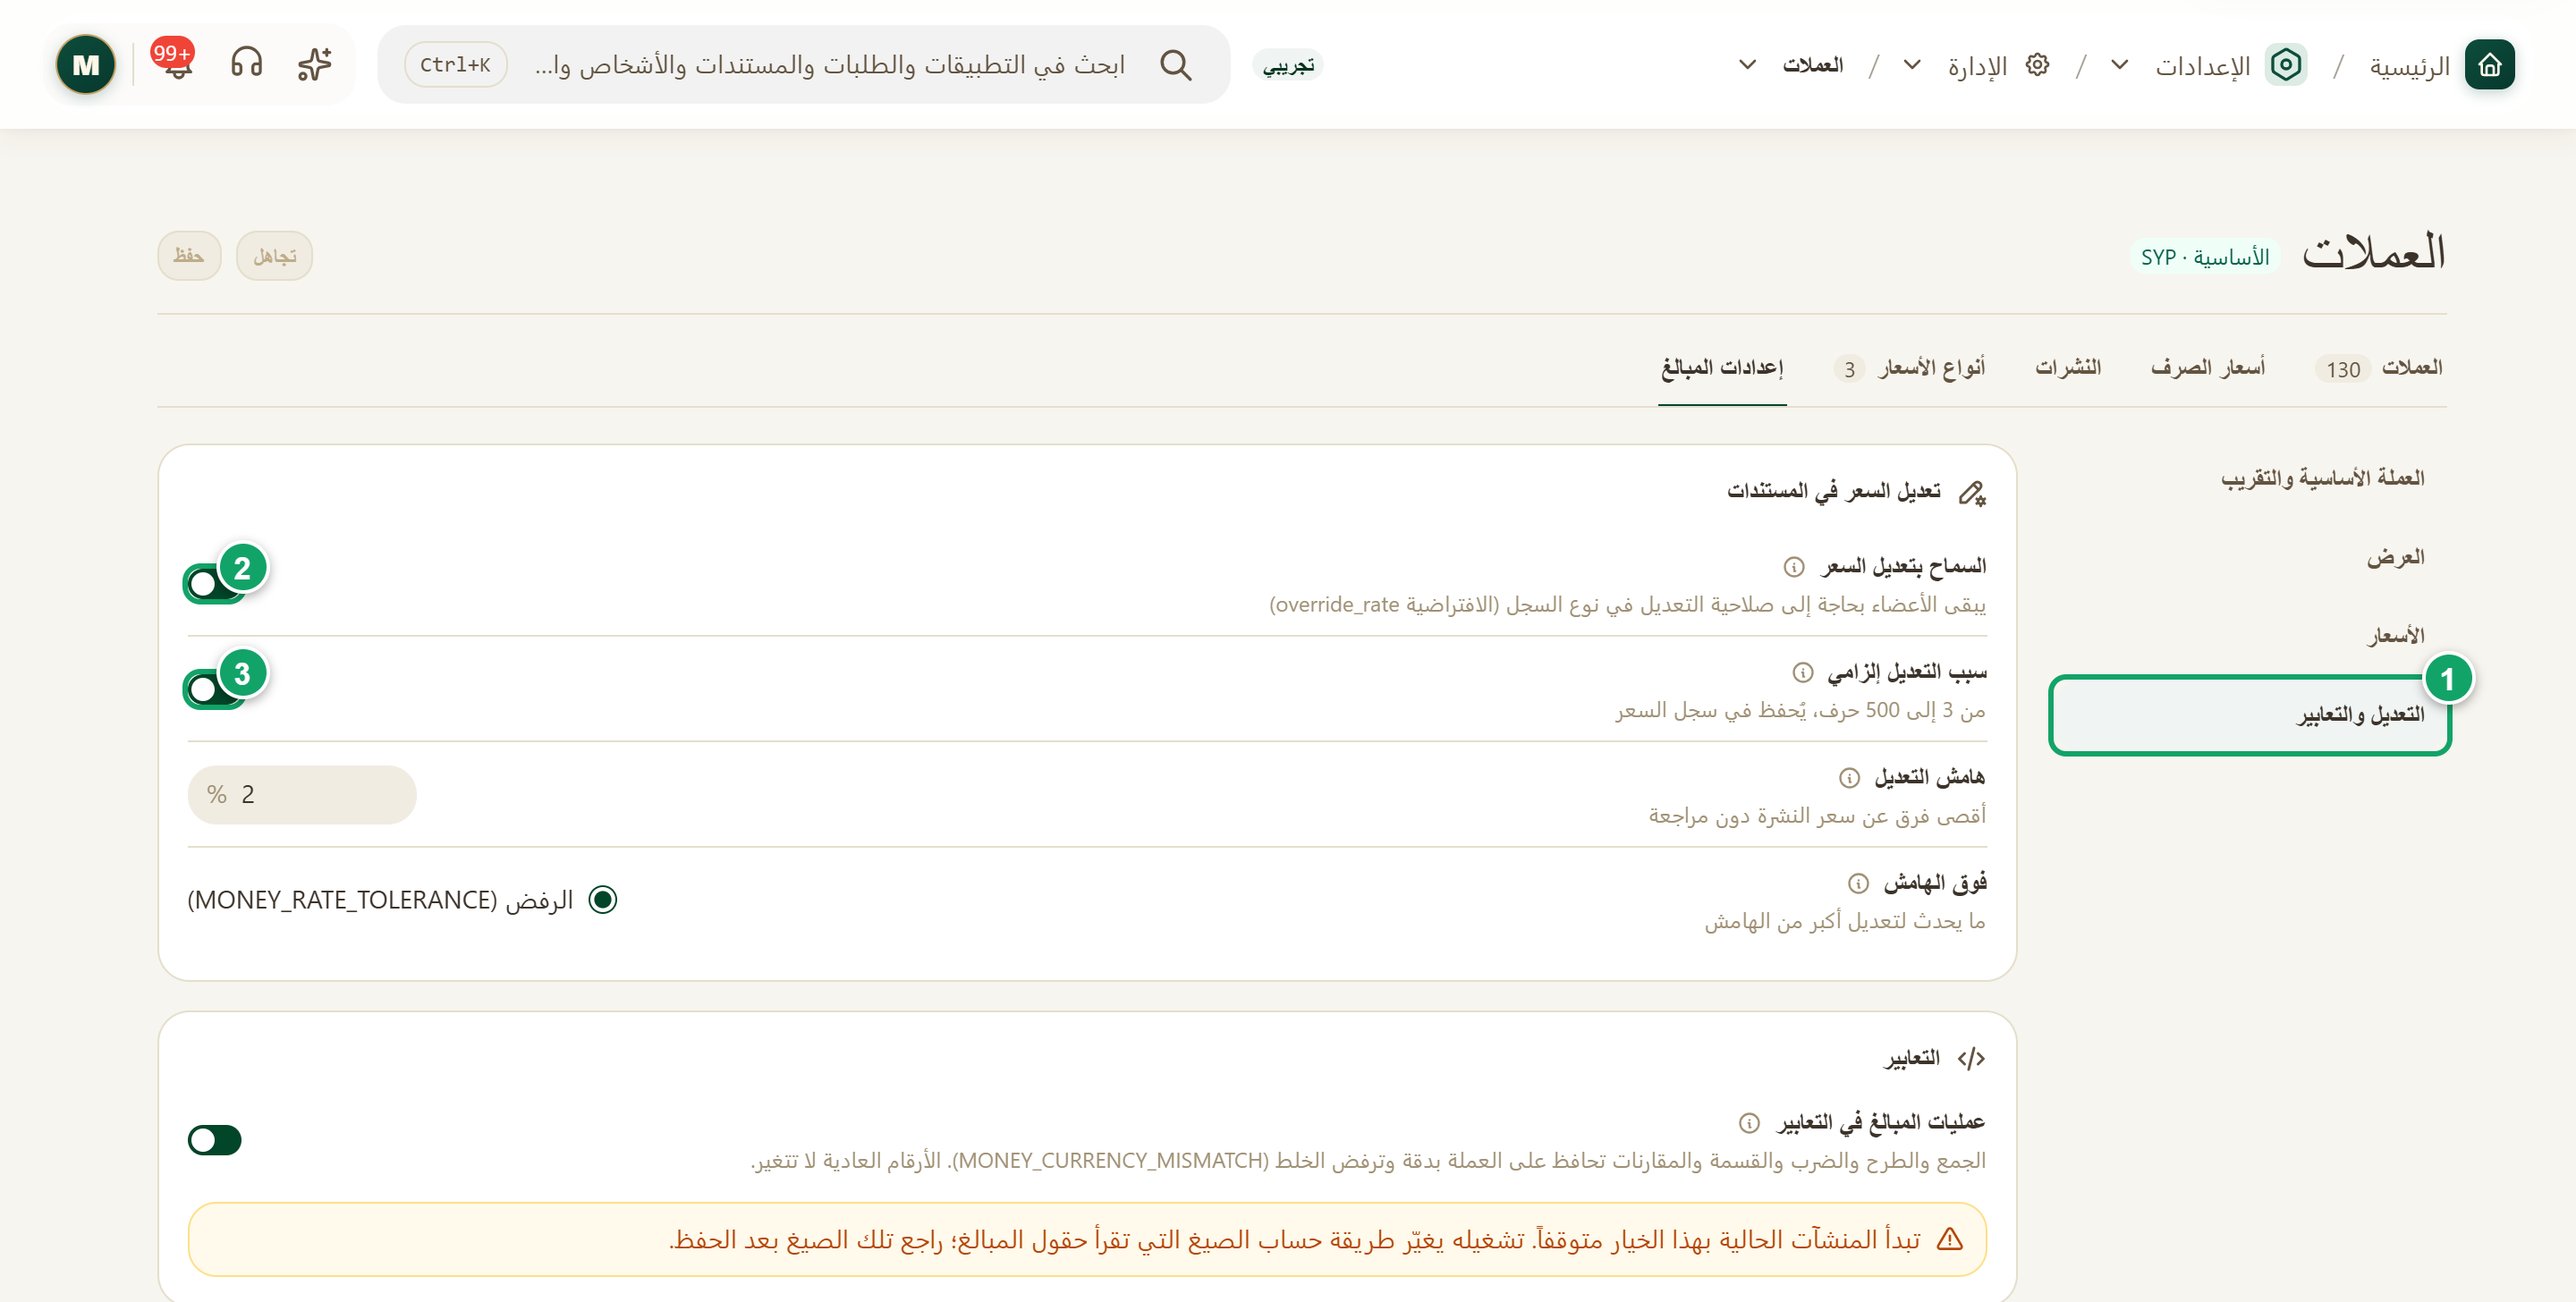
\includegraphics[width=0.95\linewidth,height=0.72\textheight,keepaspectratio]{figures/screens/ch08-currencies-settings-overrides-ar.png}
\caption{إعدادات المبالغ: التعديل والتعابير}
\label{fig:settings-currencies-settings-overrides-screen}
\shotnote{يحدد هذا القسم إن كان يجوز للعضو تعديل السعر داخل مستند، وبأي حد. والسماح هنا لا يكفي وحده؛ فالعضو يحتاج أيضاً إلى صلاحية التعديل في نوع السجل. ① «التعديل والتعابير». ② «السماح بتعديل السعر». ③ «سبب التعديل إلزامي»: يبقى السبب في سجل السعر.}
\end{figure}

\begin{table}[H]
\centering
\caption{ماذا تضبط في إعدادات المبالغ؟}
\label{tab:settings-currencies-money}
\begin{tabularx}{\linewidth}{R{4.2cm} Y}
\rcHeaderRow
\thh{القسم} & \thh{ما يمكنك ضبطه}\\
«العملة الأساسية والتقريب» & العملة الأساسية، و«طريقة التقريب»، و«مرحلة التقريب»، و«مكافئ السطور»، و«هامش توازن الطرفين بالأساسية» للمستندات ذات الطرفين.\\
«العرض» & «الأرقام في الطباعة»، و«فاصل الآلاف والكسور»، و«عرض المبالغ السالبة»، و«عرض رمز العملة»، و«المكافئ في المستندات».\\
«الأسعار» & «نوع السعر الافتراضي»، و«سعر اليوم المعتمد»، و«منازل السعر المعروضة»، و«استخدام الزوج المقلوب»، و«السعر التقاطعي عبر»، و«تحذير القفزة»، وما يحدث عند غياب السعر أو قِدمه.\\
«التعديل والتعابير» & «السماح بتعديل السعر»، و«سبب التعديل إلزامي»، و«هامش التعديل»، و«فوق الهامش»، و«عمليات المبالغ في التعابير».\\
\end{tabularx}
\end{table}

\begin{enumerate}
\item افتح «الإعدادات» ثم «العملات».
\item افتح قائمة العملة واضغط «تعديل» لتفعيل العملة أو ضبطها، أو اضغط «إضافة عملة» إذا لم تكن موجودة.
\item افتح «إعدادات المبالغ» وراجع العملة الأساسية قبل أول استخدام، لأنها تُقفل بعده.
\item افتح «أسعار الصرف» واضغط «إضافة سعر»، ثم اختر النوع والعملة والتاريخ واكتب السعر واضغط «حفظ السعر».
\item عند تغيير «إعدادات المبالغ»، اضغط «حفظ» أعلى الصفحة. يعيدك «تجاهل» إلى القيم المحفوظة.
\end{enumerate}

\textbf{تحقق:} تظهر العملة بحالة «نشط» في القائمة، ويظهر السعر الجديد في «الأزواج · آخر سعر» وفي عمود السعر. إذا أخطأت في سعر، فلا تبحث عن زر تعديل: افتح إجراءات السعر واستخدم «تصحيح…». وإذا أخبرك تبويب «النشرات» بأنه لا يوجد نوع سعر يقبل النشرات، فافتح «أنواع الأسعار» واضبط «تأتي الأسعار» على «في نشرات».

\section{وحدات القياس}
\label{sec:settings-feature-units}

تحدد هذه الصفحة الوحدات التي يختار منها الأعضاء في أسئلة الكميات والنسب والمصفوفات وفي حقول السجلات، مثل الكيلوغرام واللتر. وتُجمع الوحدات في مجموعات، وإذا كانت وحدات المجموعة قابلة للتحويل فلها «وحدة أساس» تتحول إليها البقية، فيستطيع النظام جمع كميات كُتبت بوحدات مختلفة. تفيدك الصفحة عندما تحتاج مؤسستك إلى وحدة غير موجودة. يفتحها من يملك صلاحية عرض الوحدات ومجموعات الوحدات.

تبدأ كل مؤسسة بوحدات من النظام، ويمكنك إعادة تسميتها أو إخفاءها دون تغيير مفتاحها أو تحويلها. أما الوحدة التي استُخدمت فيثبت تحويلها ولا تُحذف، لتبقى الإجابات المحفوظة بمعناها.

\begin{rcnote}[مثال: شركة الأفق]
تستلم شركة الأفق مواد الضيافة بالكرتونة دون وزن معروف. لذلك ينشئ مسؤول النظام مجموعة «عبوات» بنوع «بلا تحويل» عند ①، ثم يضيف إليها وحدة «كرتونة» عند ②؛ فتُجمع الكراتين وحدها ولا تختلط بالكيلوغرامات.
\end{rcnote}

\begin{figure}[H]
\centering
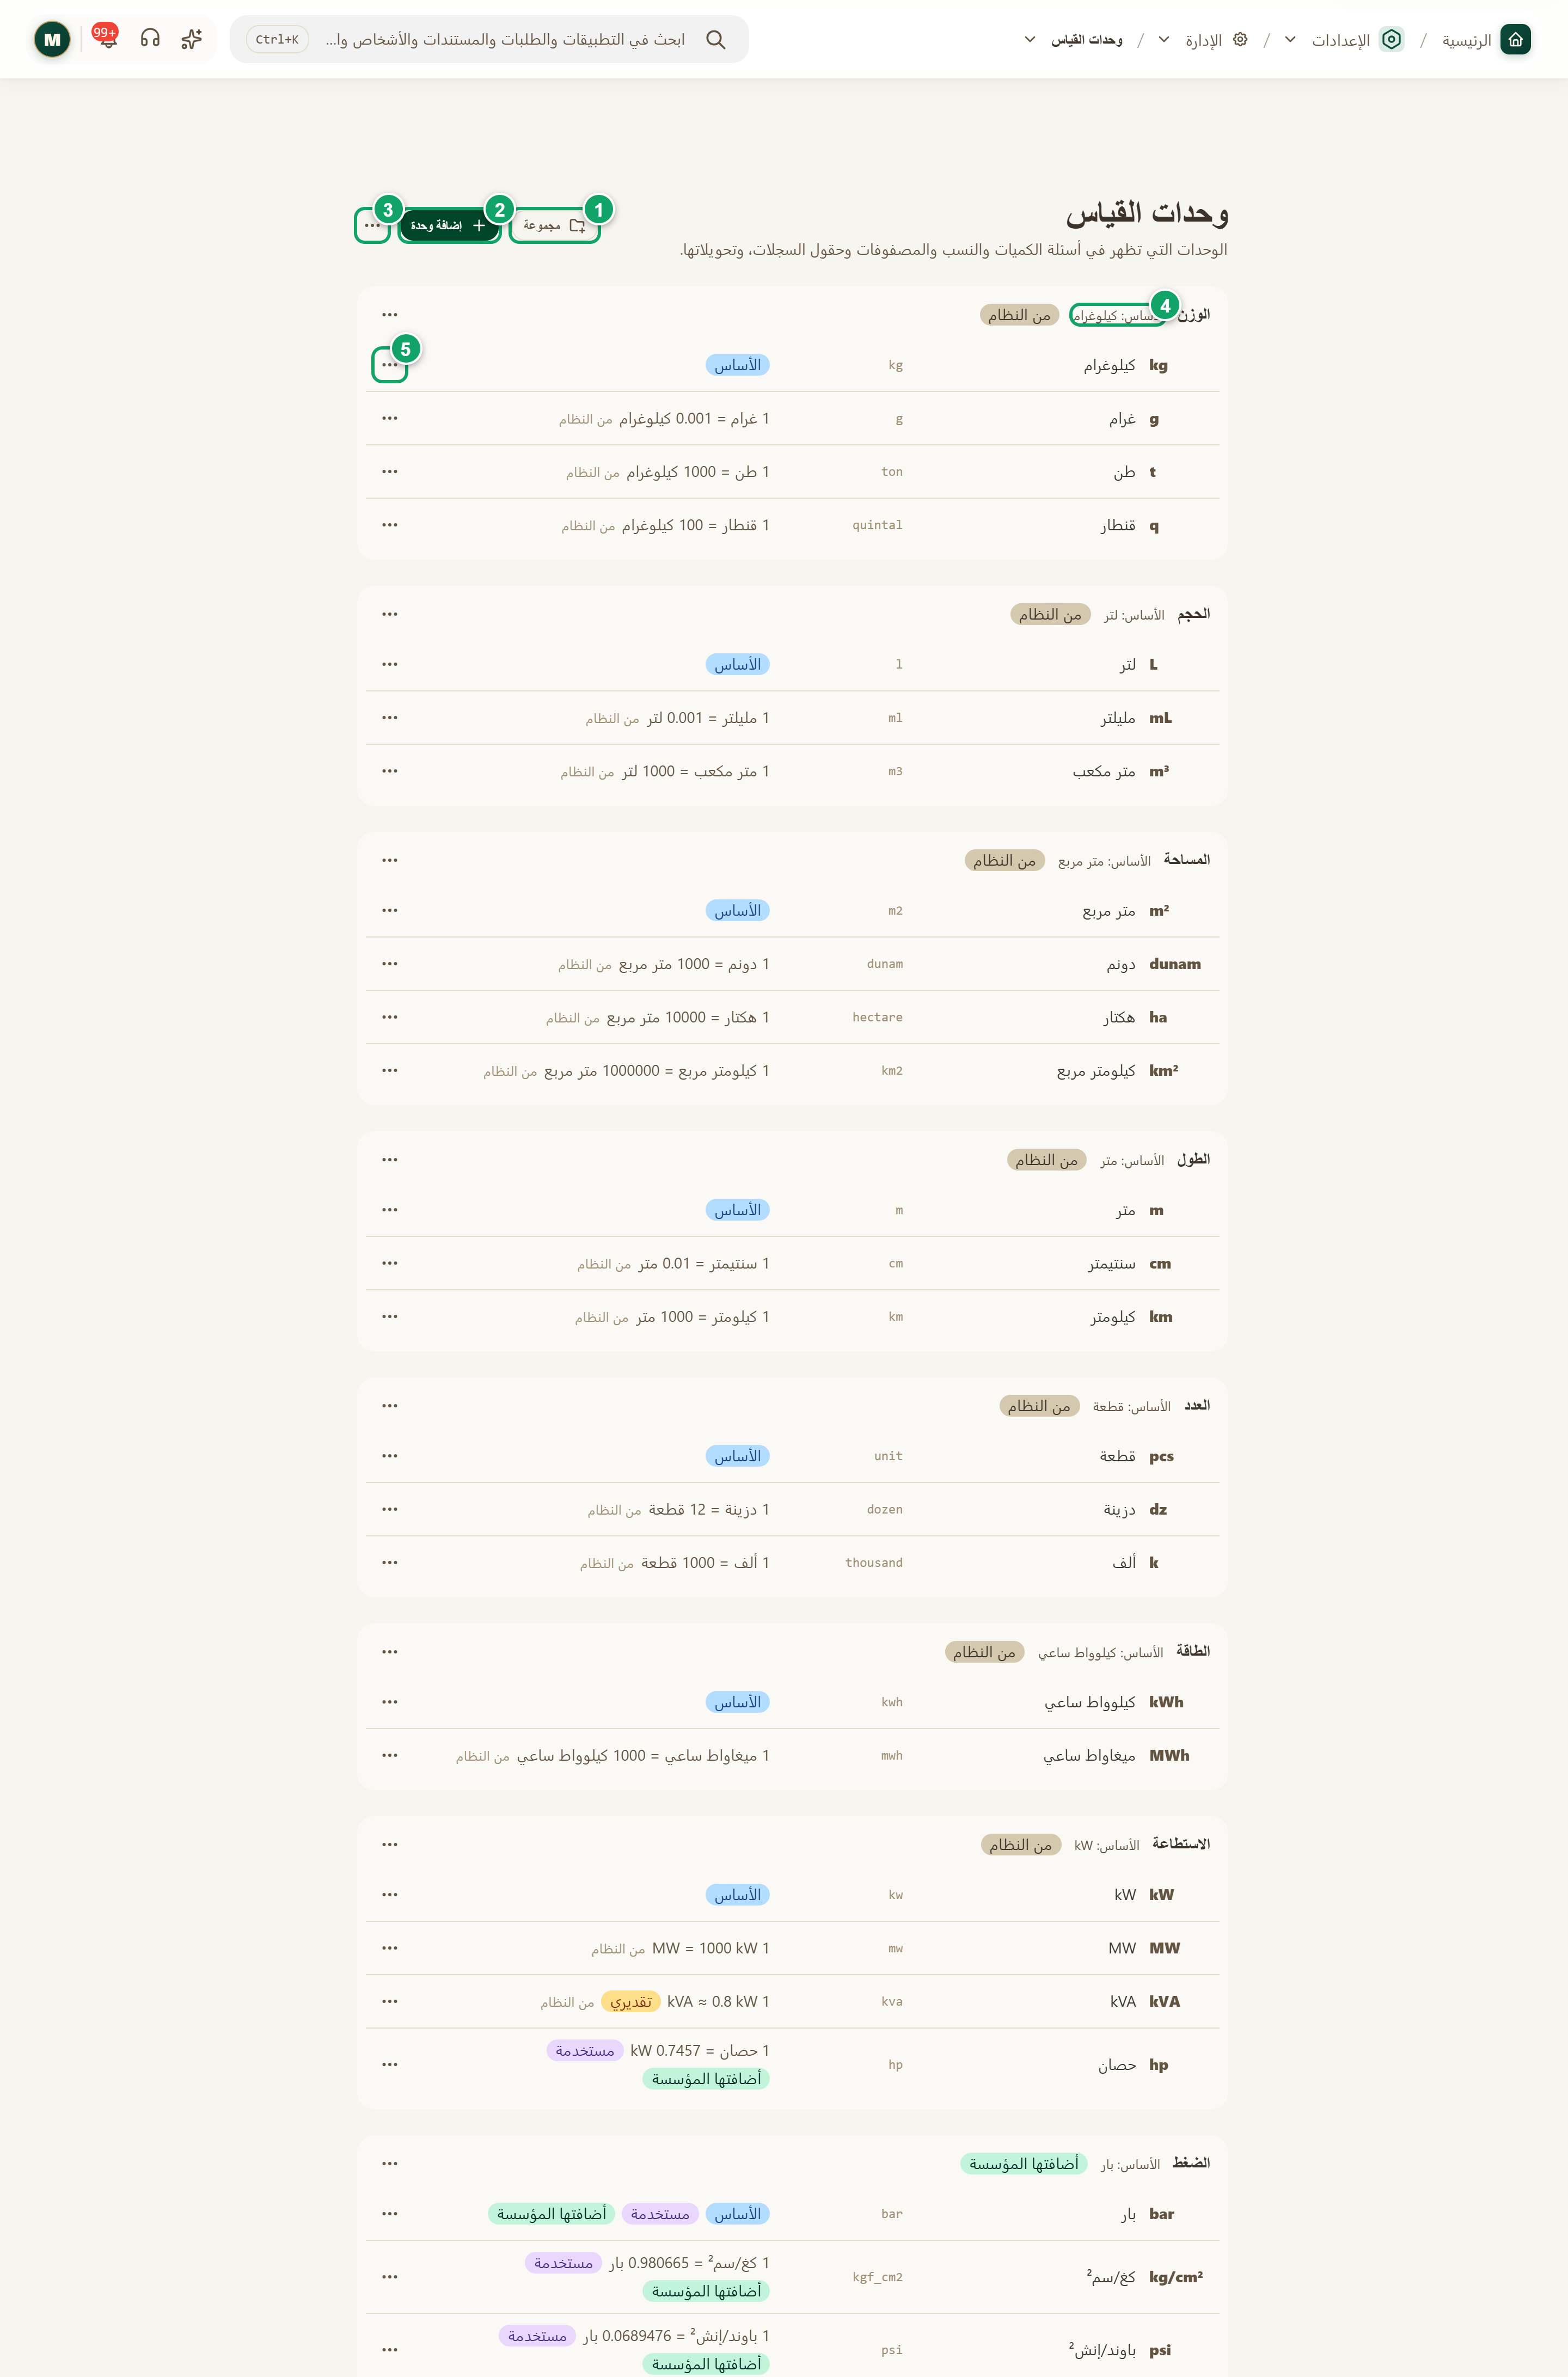
\includegraphics[width=0.95\linewidth,height=0.72\textheight,keepaspectratio]{figures/screens/ch08-units-ar.png}
\caption{مجموعات الوحدات}
\label{fig:settings-units-screen}
\shotnote{تعرض الصفحة كل مجموعة مع وحداتها وتحويل كل وحدة إلى الأساس. وتميّز الشارات مصدر الوحدة وحالتها، مثل «من النظام» و«أضافتها المؤسسة» و«مستخدمة»، فتعرف ما يمكن تغييره قبل فتحه. ① «مجموعة». ② «إضافة وحدة». ③ «إجراءات أخرى»: يفتح «استيراد وحدات». ④ وحدة أساس المجموعة. ⑤ قائمة الوحدة: «تعديل» و«إخفاء» والنقل، و«حذف» إن كانت الوحدة قابلة للحذف.}
\end{figure}

\begin{figure}[H]
\centering
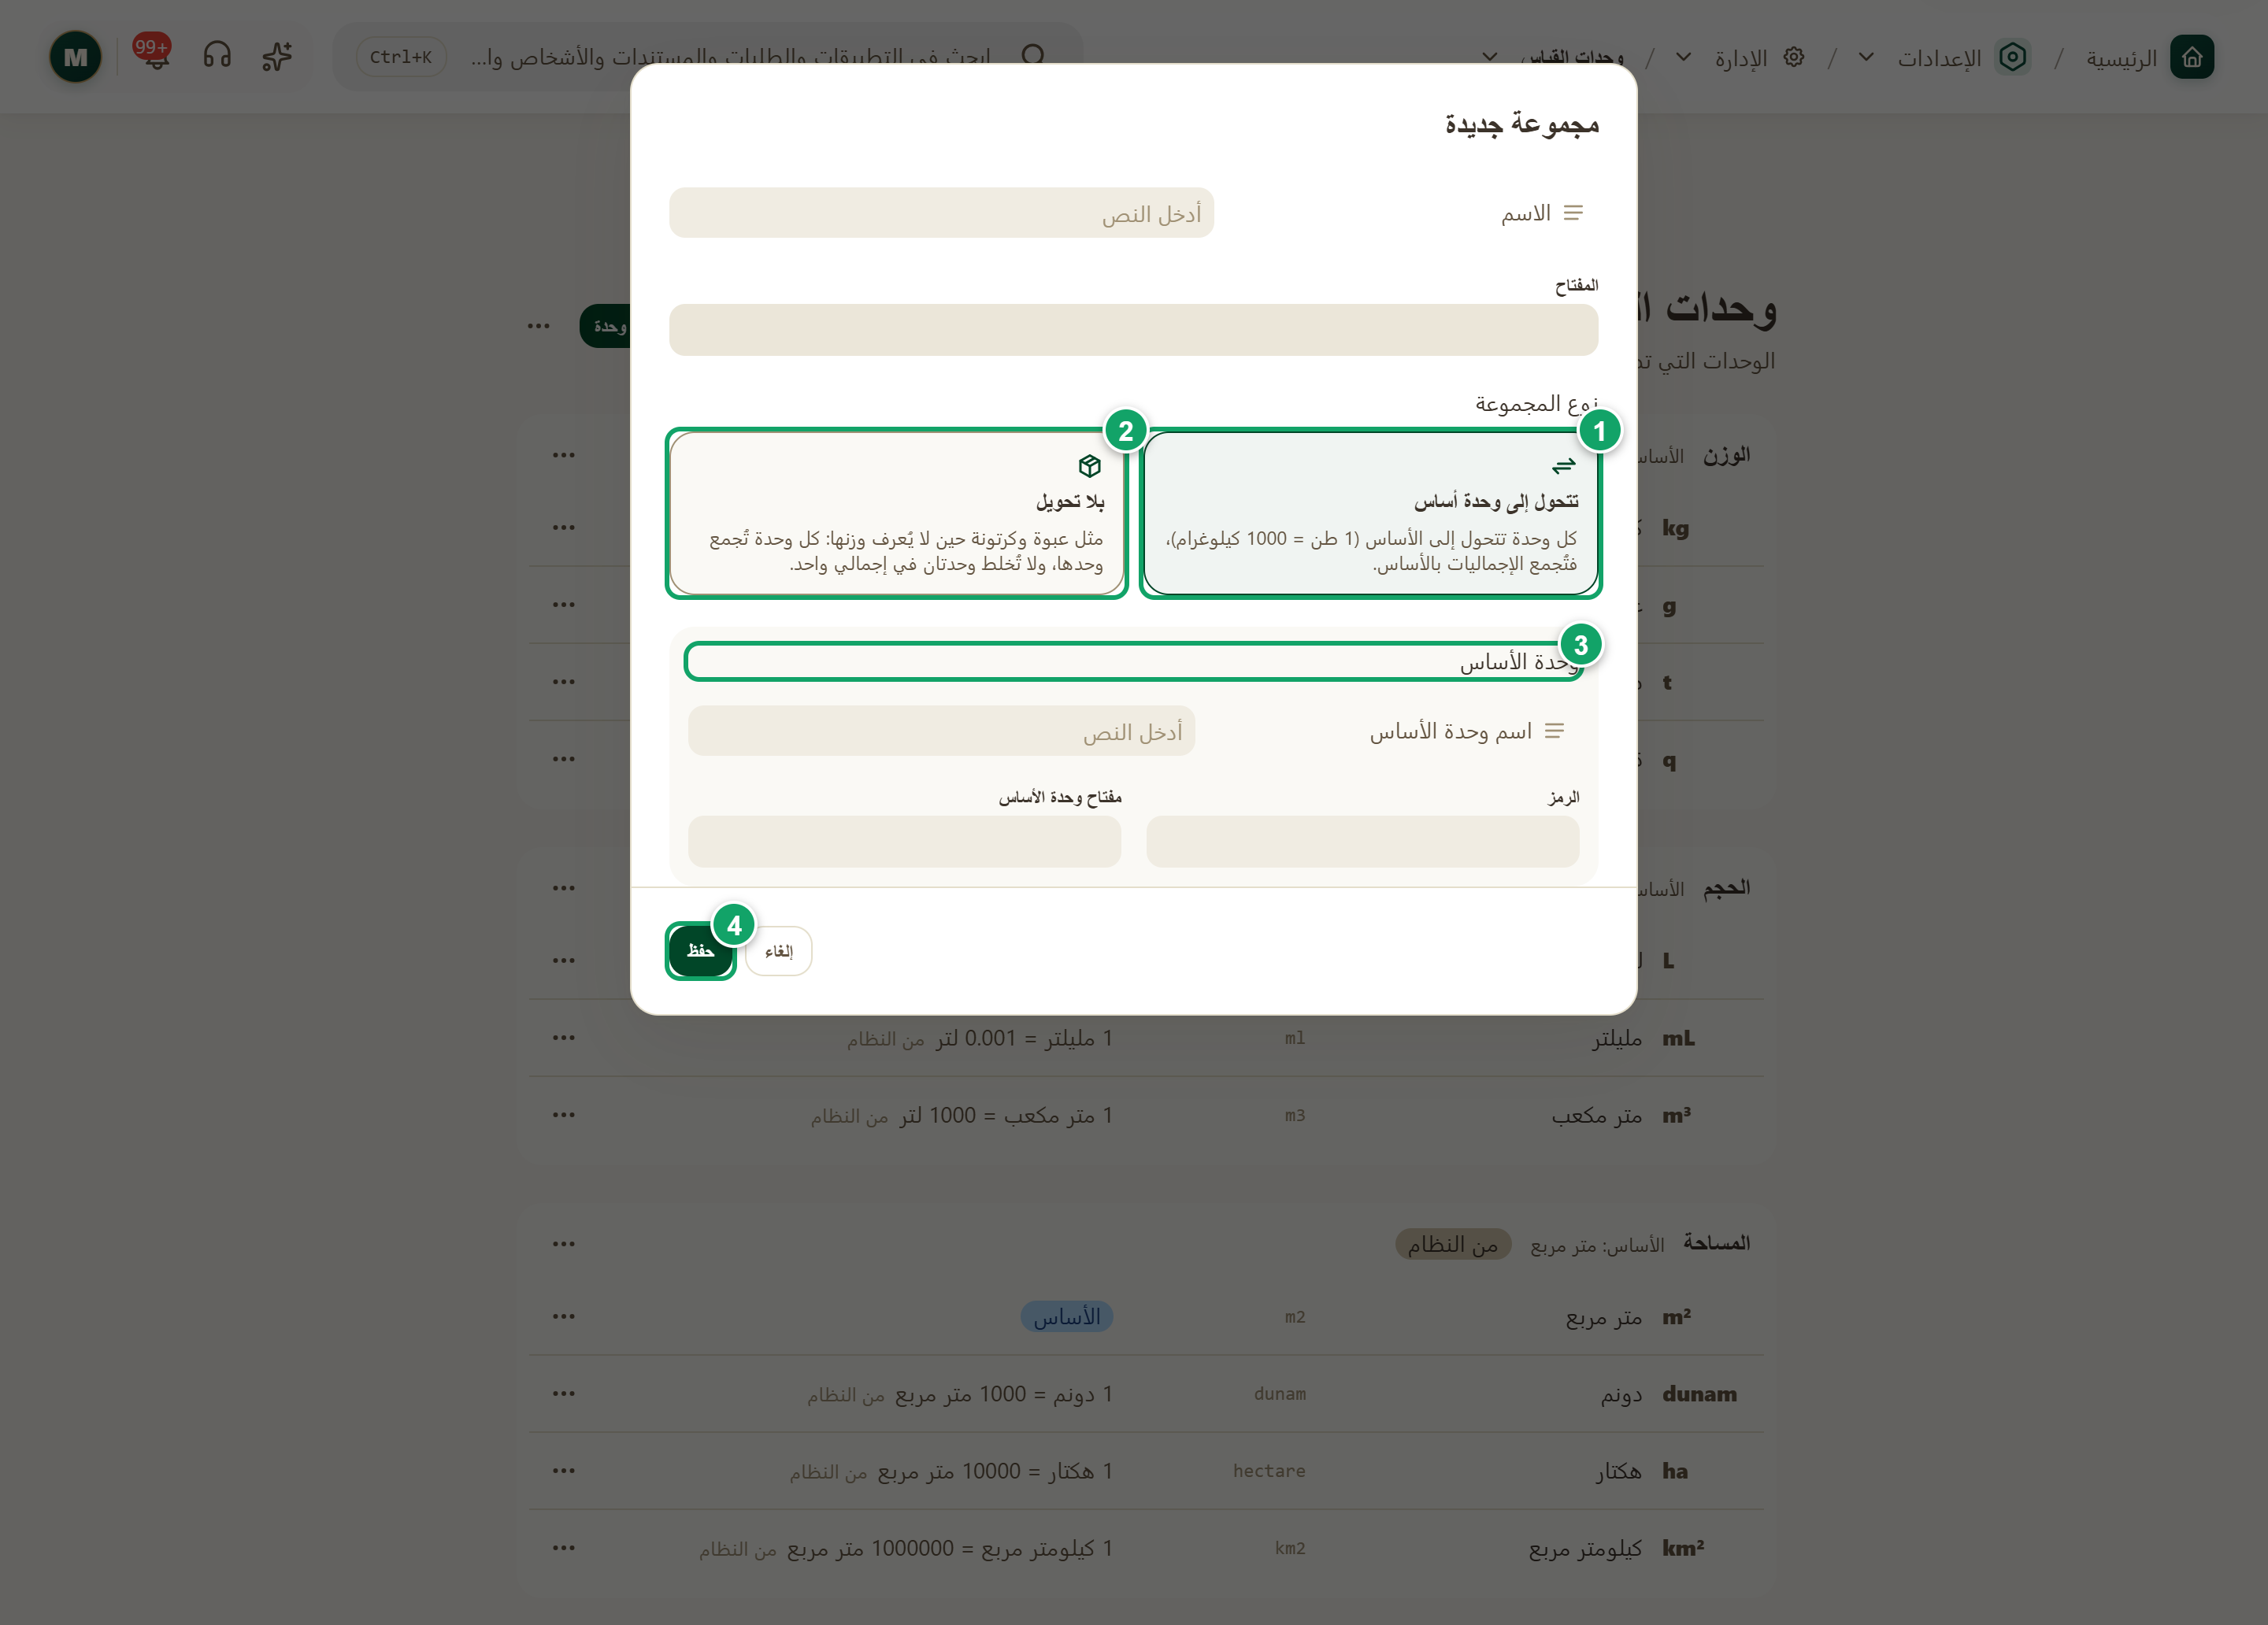
\includegraphics[width=0.95\linewidth,height=0.72\textheight,keepaspectratio]{figures/screens/ch08-units-group-ar.png}
\caption{نافذة مجموعة جديدة}
\label{fig:settings-units-group-screen}
\shotnote{يُتخذ أهم قرار عند إنشاء المجموعة، لأن نوعها ووحدة أساسها لا يتغيران بعد ذلك. والنافذة هنا فارغة ولم تُحفظ. ① «تتحول إلى وحدة أساس»: مثل 1 طن = 1000 كيلوغرام. ② «بلا تحويل»: كل وحدة تُجمع وحدها. ③ «وحدة الأساس»: اسمها ورمزها ومفتاحها. ④ «حفظ».}
\end{figure}

\begin{figure}[H]
\centering
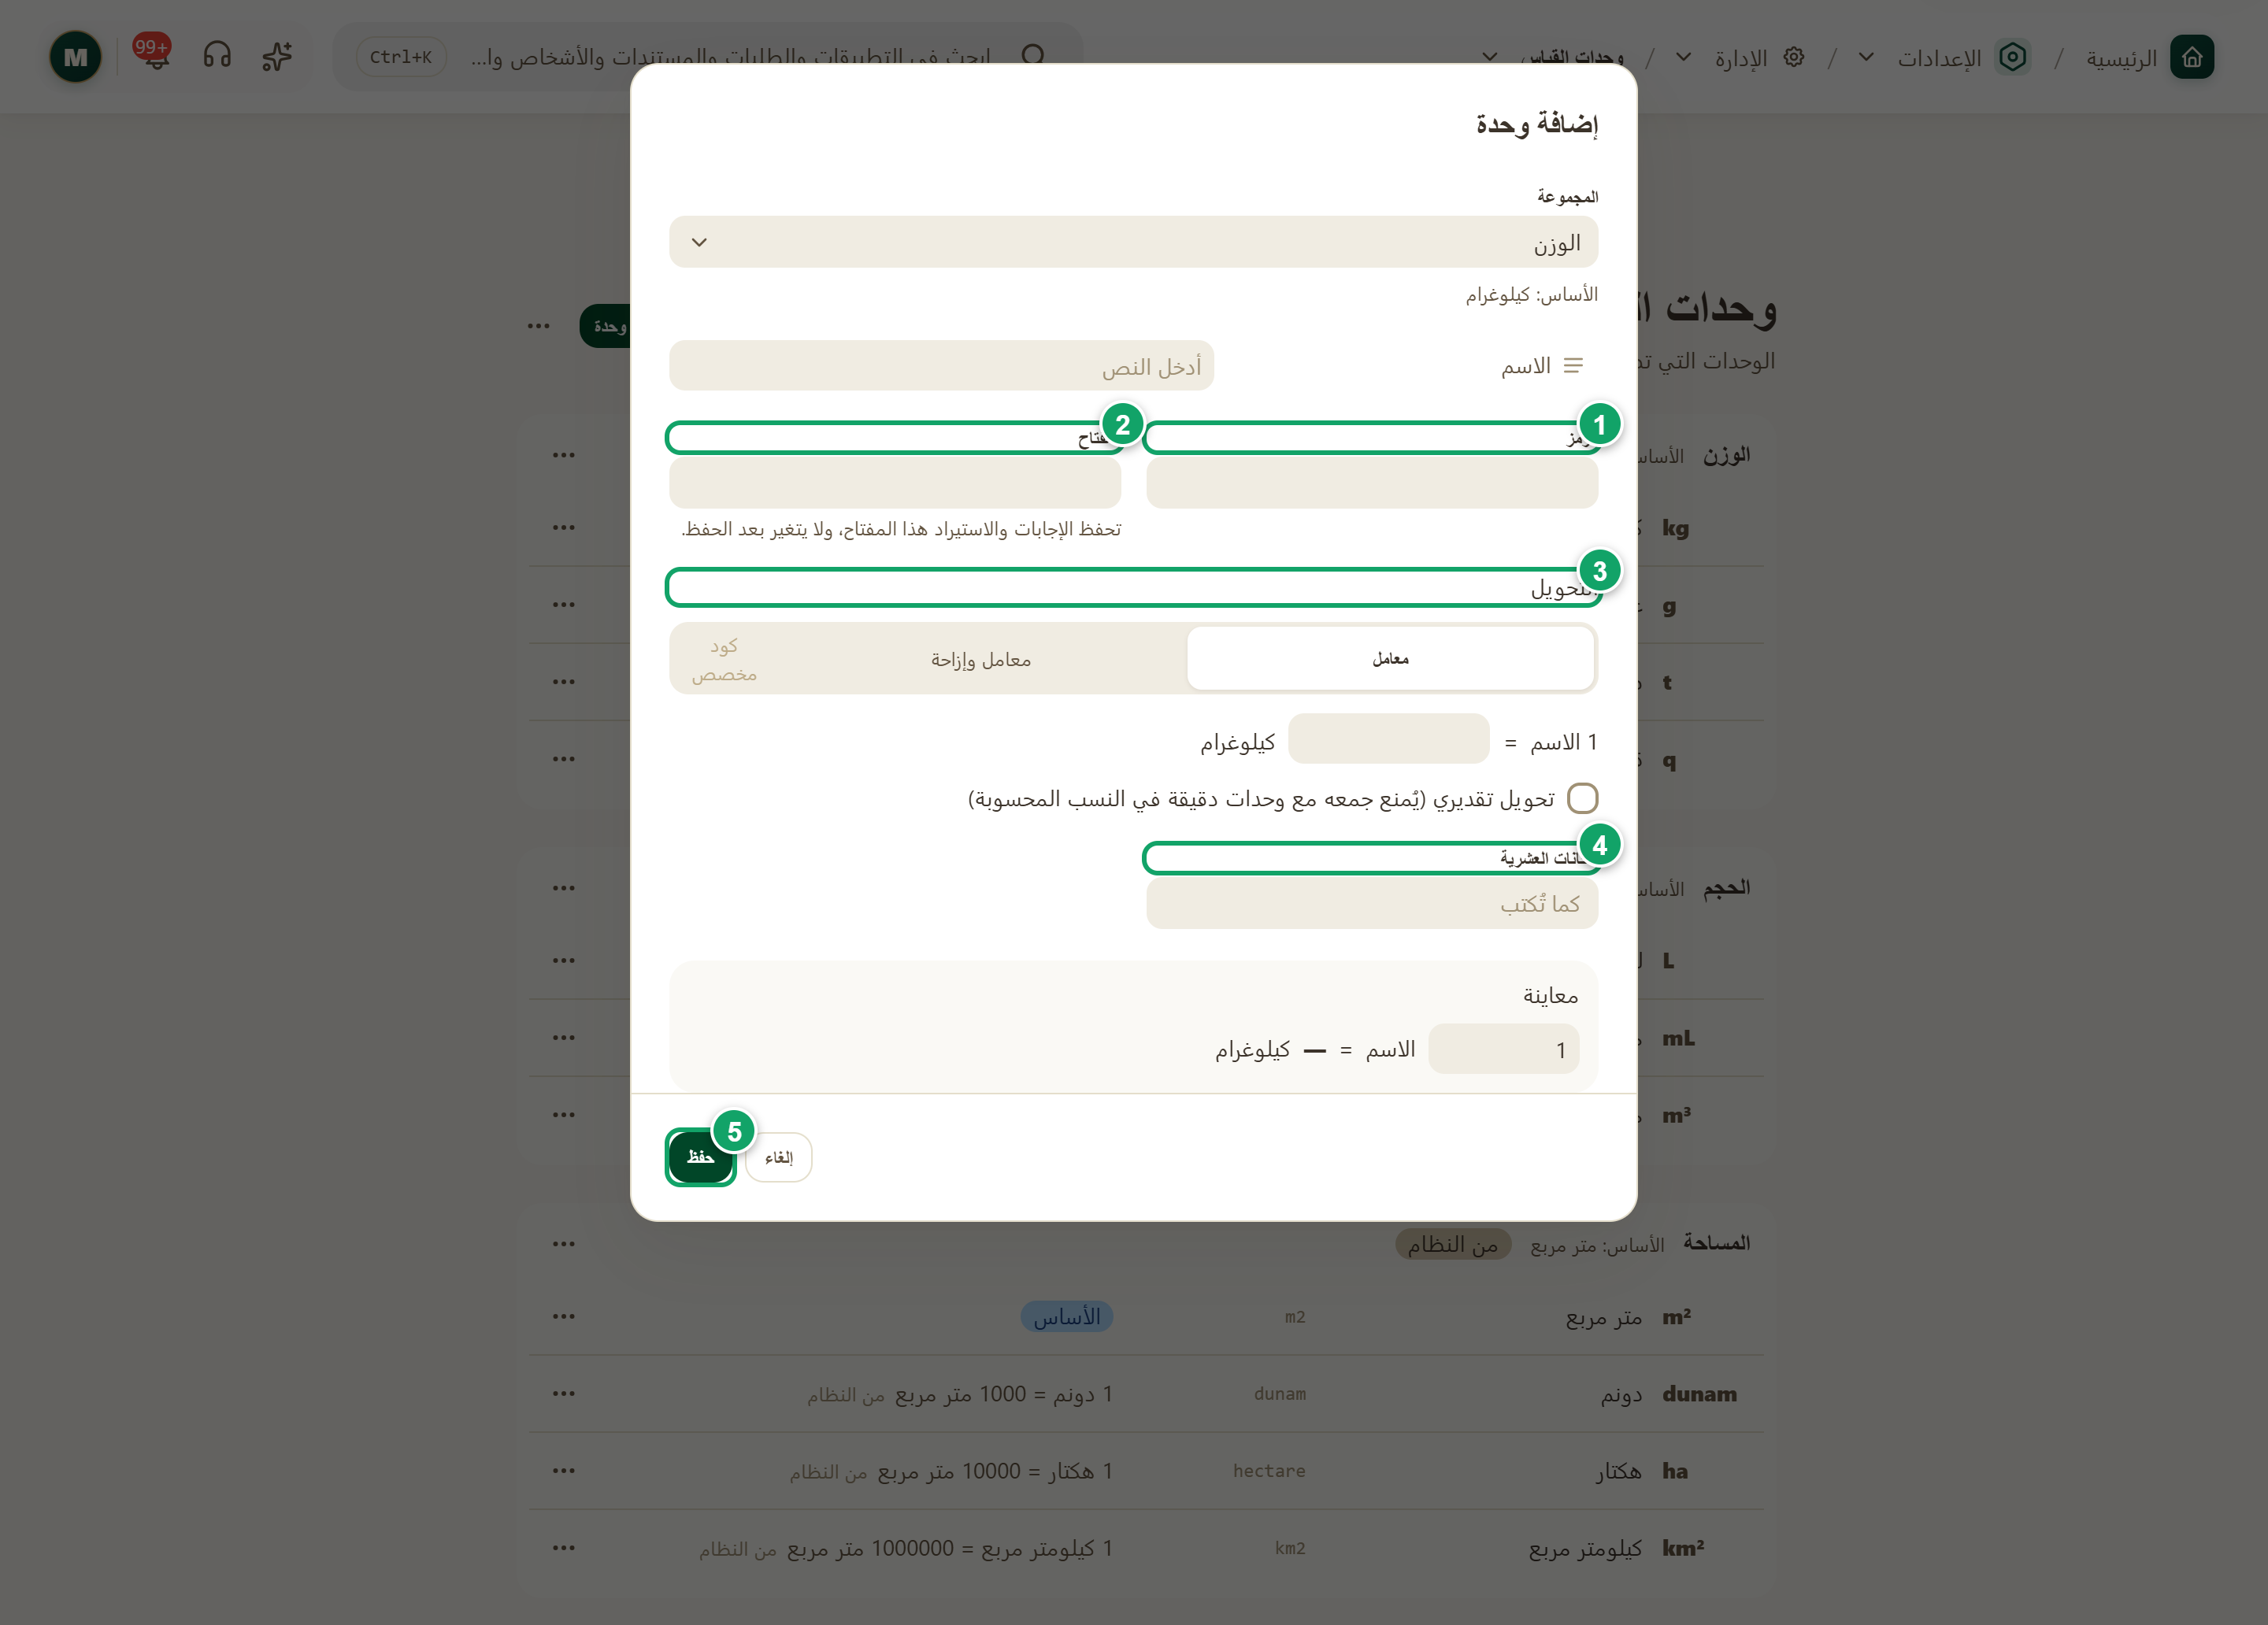
\includegraphics[width=0.95\linewidth,height=0.72\textheight,keepaspectratio]{figures/screens/ch08-units-form-ar.png}
\caption{نافذة إضافة وحدة}
\label{fig:settings-units-form-screen}
\shotnote{تحدد النافذة اسم الوحدة ومقدارها بالنسبة إلى وحدة الأساس، وتعرض معاينة تساعدك على التأكد من التحويل قبل الحفظ. ① «الرمز». ② «المفتاح»: يُملأ من الاسم ولا يتغير بعد الحفظ. ③ «التحويل». ④ «الخانات العشرية». ⑤ «حفظ».}
\end{figure}

\begin{table}[H]
\centering
\caption{ماذا تسجل في الوحدة والمجموعة؟}
\label{tab:settings-units-fields}
\begin{tabularx}{\linewidth}{R{4.2cm} Y}
\rcHeaderRow
\thh{الحقل} & \thh{ماذا يعني؟}\\
«المجموعة» & المجموعة النشطة التي تنتمي إليها الوحدة.\\
«الاسم» و«الرمز» & الاسم بكل لغة نشطة، والاختصار الظاهر بجانب الكمية.\\
«المفتاح» & اسم ثابت تحفظه الإجابات والاستيراد، يبدأ بحرف ويستخدم a–z و0–9 و\_ فقط.\\
«التحويل» & «معامل» مثل 1 طن = 1000 كيلوغرام، أو «معامل وإزاحة» للوحدات التي لا تبدأ من الصفر. وخيار «كود مخصص» غير متاح بعد.\\
«تحويل تقديري» & يوضع على التحويل غير الدقيق، فلا يُخلط مع الوحدات الدقيقة عند حساب النسب.\\
«الخانات العشرية» & عدد صحيح من 0 إلى 10، أو «كما تُكتب».\\
«الكلمات عند الطباعة» & يظهر عند تعديل وحدة محفوظة، ويضبط صيغ الاسم عند طباعة الرقم بالحروف.\\
\end{tabularx}
\end{table}

\begin{enumerate}
\item افتح «الإعدادات» ثم «وحدات القياس».
\item إذا لزمت مجموعة جديدة، فاضغط «مجموعة»، واكتب «الاسم»، واختر نوعها، ثم اضغط «حفظ».
\item افتح قائمة المجموعة واضغط «إضافة وحدة إلى هذه المجموعة»، أو اضغط «إضافة وحدة» واختر المجموعة.
\item اكتب «الاسم» و«الرمز»، ثم اكتب المعامل إذا كانت المجموعة تتحول، واضغط «حفظ».
\item لإزالة وحدة لم تُستخدم، افتح قائمتها واضغط «حذف» ثم أكد. أما الوحدة المستخدمة فاضغط «إخفاء» بدلاً من ذلك.
\end{enumerate}

\textbf{تحقق:} تظهر الوحدة داخل مجموعتها بشارة «أضافتها المؤسسة»، وتبقى كذلك بعد إعادة تحميل الصفحة، ويظهر تحويلها بجانبها. أعد فتحها من «تعديل» لتجد «المفتاح» مقفلاً. وعند حذف مجموعة تُحذف وحداتها معها ما دامت لم تُستخدم.
